% =========================================================================
%  Project report — single-file setup.
%  Operational State Recognition and Braking Behaviour Analysis
%  for Predictive Maintenance on Metro Trains
%
%  Compile with:  pdflatex -> biber -> pdflatex -> pdflatex
% =========================================================================
\documentclass[11pt,a4paper,twoside]{report}

% ---------- encoding & fonts ----------
\usepackage[T1]{fontenc}
\usepackage[utf8]{inputenc}
\usepackage{lmodern}
\usepackage{microtype}
\usepackage[english]{babel}

% ---------- page geometry ----------
\usepackage[a4paper,inner=3.0cm,outer=2.5cm,top=2.7cm,bottom=2.7cm]{geometry}
\usepackage{setspace}
\onehalfspacing

% ---------- discourage widows / orphans ----------
\clubpenalty=10000
\widowpenalty=10000
\displaywidowpenalty=10000

% ---------- maths, units, tables ----------
\usepackage{amsmath,amssymb}
\usepackage{siunitx}
\sisetup{output-decimal-marker={.},range-phrase={--},group-separator={\,}}
\usepackage{booktabs}
\usepackage{caption}
\usepackage{etoolbox}
\usepackage{titlesec}

\captionsetup{skip=10pt}
\usepackage{tabularx}
\usepackage{ragged2e}
\usepackage{multirow}

% ---------- graphics ----------
\usepackage{graphicx}
\graphicspath{{Bilder/}}
\usepackage{xcolor}
\definecolor{linkblue}{HTML}{264B96}

% ---------- quotations ----------
\usepackage[autostyle,english=american]{csquotes}

% ---------- bibliography ----------
\usepackage[style=numeric-comp,backend=biber,maxcitenames=2,maxbibnames=99,giveninits=true]{biblatex}
\addbibresource{Literatur.bib}

% ---------- headers / footers: page number on EVERY page ----------
\usepackage{fancyhdr}
\pagestyle{fancy}
\fancyhf{}
\fancyhead[LE]{\small\nouppercase{\leftmark}}
\fancyhead[RO]{\small\nouppercase{\rightmark}}
\fancyfoot[C]{\thepage}
\renewcommand{\headrulewidth}{0.4pt}
\renewcommand{\footrulewidth}{0pt}
% chapter-opening pages ("plain") also carry the footer page number
\fancypagestyle{plain}{%
  \fancyhf{}%
  \fancyfoot[C]{\thepage}%
  \renewcommand{\headrulewidth}{0pt}%
}

% ---------- blank filler pages carry no header/footer ----------
\usepackage{emptypage}

% ---------- hyperlinks (load last) ----------
\usepackage[colorlinks=true,linkcolor=linkblue,citecolor=linkblue,urlcolor=linkblue]{hyperref}

% ---------- title metadata ----------
\newcommand{\thetitleEN}{Operational State Recognition and Braking Behaviour Analysis for Predictive Maintenance on Metro Trains}
\newcommand{\figspace}{\vspace{0.5cm}}

\titleformat{\chapter}[hang]
  {\normalfont\Huge\bfseries}{\thechapter}{0.6em}{}
\titlespacing*{\chapter}{0pt}{0pt}{20pt}

\begin{document}

% =========================================================================
%  Title page
% =========================================================================
\begin{titlepage}
\centering
\thispagestyle{empty}
\noindent\hspace*{-1.5cm}%
\begin{minipage}[c]{0.5\textwidth}
    \centering
    
\includegraphics[height=1.35cm]{R.png}
\end{minipage}%
\hfill
\begin{minipage}[c]{0.5\textwidth}
    \centering
    
\includegraphics[height=2.7cm]{imw_logo-1.png}
\end{minipage}
\hspace*{-1.5cm}


\vspace*{1.5cm}
{\scshape\large Technische Universit\"at Wien\par}
\vspace{0.3cm}
{\scshape Interdisciplinary Project Report\par}
\vspace{1.7cm}
\rule{\linewidth}{0.4pt}\par
\vspace{0.9cm}
{\LARGE\bfseries \thetitleEN \par}
\vspace{0.9cm}
\rule{\linewidth}{0.4pt}\par
\vspace{1.7cm}
{\large\bfseries Maximilian Scheiblauer, BSc\par}
{\normalsize Matriculation Number 11776651\par}
\vspace{2cm}
{\normalsize
\begin{tabular}{r l}
Supervisors: & Dipl.-Ing.\ Andreas Steiner, Institut f\"ur Managementwissenschaften \\
             & Dr.\ Florina Piroi, Institut f\"ur Information Systems Engineering \\
\end{tabular}\par}
\vspace{1cm}
{\large July 2026\par}
\end{titlepage}

% =========================================================================
%  Front matter — roman page numbers
% =========================================================================


% single-space the TOC so title page + contents stay within two pages
\begingroup
\singlespacing
\tableofcontents
\endgroup

% =========================================================================
%  Main matter — arabic page numbers, restart at 1
% =========================================================================

\pagenumbering{arabic}
\setcounter{page}{0}

\chapter{Introduction}
\label{ch:introduction}
Much rail maintenance still runs on fixed intervals: a component is inspected or replaced after
a set mileage or time, regardless of how hard it has actually been used. That wastes healthy
parts and still misses parts that fail early under unusual load. Predictive maintenance ties
each intervention to the measured condition of the equipment instead, promising less wasted
material and fewer unnecessary replacements. The friction brakes of a metro train are a good
place to try this: the train brakes at almost every stop, hundreds of times a day, so the brake
components are cycled constantly and any degradation should leave a large, repeating signal.
This report analyses the MetroAT dataset~\cite{MetroAT:2026}: one year of 1\,Hz recordings from a
single Wiener Linien metro train, covering the pneumatic system together with train speed and mode
signals, and annotated with documented failure and maintenance events. All sensor values are
min-max normalised, so the analysis works in relative rather than physical units. Following the
project proposal, the work runs in two phases along the CRISP-DM cycle~\cite{WirthHipp:00}. The first recognises the
train's operational regimes without supervision, clustering the motion signal into a small set of
interpretable states. The second examines the braking that dominates mechanical wear: individual
deceleration events are extracted, their intensity characterised, and braking behaviour tested for
any trend ahead of documented brake-system failures.

Four questions run through the report: (1) whether distinct operational regimes emerge from the
motion data alone, without fixing their number in advance; (2) given those regimes, whether the
air-system sensors can recover the deceleration regime using only signals that did not help define
it; (3) whether deceleration intensity falls into discrete classes or forms a continuum, and how
much of it the air-system sensors can explain; and (4) whether braking behaviour carries any
detectable signal ahead of documented brake-system failures. The remainder of the report is organised by topic rather than by project phase.

\textbf{Structure.} Chapter~\ref{ch:preprocessing} describes how the raw recordings become the
analysis units and how the sensors are partitioned into feature roles.
Chapter~\ref{ch:states} derives and validates four motion-only operational states.
Chapter~\ref{ch:classification} tests whether the air-system sensors alone can recover the
deceleration state. Chapter~\ref{ch:braking} extracts individual deceleration events and regresses
their intensity and dissipated energy from the air sensors. Chapter~\ref{ch:failure} examines the
link to documented failures and the maintenance calendar and reports a near-null pre-failure
result. Chapter~\ref{ch:conclusion} draws the findings together and points to what is worth doing
next.

\textbf{Scope.} The conclusions are bounded by the data: a single train, an eight-and-a-half-month
training window, and roughly ten documented failures, eight of them brake-system failures; the
study is exploratory and not meant as a deployable failure detector. Differences between individual
wagons are not analysed: the many near-duplicate per-wagon channels are instead collapsed by
principal component analysis during preprocessing (Chapter~\ref{ch:preprocessing},
Figure~\ref{fig:pca}).
\chapter{Preprocessing}
\label{ch:preprocessing}

This chapter describes how the raw MetroAT recordings became the units of analysis, and
the design choices along the way that affect every later result.

\section{The dataset}

MetroAT~\cite{MetroAT:2026} is delivered as Parquet, so no conversion from CSV was needed.
The schema has 109 columns: 74 continuous sensor channels, 20 binary channels, 7
operational-mode signals, 4 failure and maintenance markers, and 4 timestamp columns. The
recordings run at 1\,Hz over roughly one year.

Several properties of the data shaped the processing:

\begin{itemize}
  \item \textbf{Normalised values.} All sensor channels are min-max normalised to
        approximately $[0,1]$; they are not physical units. Every threshold used in this
        study is therefore empirical or quantile-based, and no number in this report should
        be read as bar, \si{\metre\per\second\squared}, or \si{\kilo\pascal}.
  \item \textbf{Unsorted rows.} Rows are not guaranteed to be time-sorted within a daily
        file, so each file is sorted on load before any derivative is computed.
  \item \textbf{Streaming.} The data is processed one daily file at a time, keeping peak
        memory below 4\,GB rather than loading the full year at once.
  \item \textbf{Per-wagon replication.} Many pneumatic channels are duplicated across
        wagons, producing 214 sensor pairs with $|r| > 0.98$. No columns are deleted by
        hand. Instead, where a compact input is needed, principal component analysis is
        applied to the pneumatic set and the leading components are used in place of the raw
        channels; because so many channels are near-duplicates, a handful of components
        already captures most of the variance (Figure~\ref{fig:pca}).
\end{itemize}

\section{Train and held-out split}
\label{sec:split}

Models are fitted on a training window (June 2024 to 11 February 2025, about 14.3~million
rows) and scored on a held-out window from 12 February to June 2025 that the models never
see during fitting. Every out-of-sample figure reported later therefore comes from the
held-out window. The training window contains 10 documented failures and 11 maintenance
events, 8 of the failures being brake-system failures; these small counts are what make the
pre-failure analysis of Chapter~\ref{ch:failure} exploratory rather than conclusive.

\section{Windowing}
\label{sec:windowing}

The unit of analysis is a non-overlapping ten-second window. The roughly 30~million raw
rows reduce to about 1.49~million windows. For each window, summary statistics are computed
per channel (means and standard deviations, and minima and maxima for the kinematic
channels), so that each window carries a compact description of both motion and
air-system behaviour over its ten seconds. The ten-second choice is a compromise between
resolution and stability; its robustness is examined directly in
Section~\ref{sec:window-sensitivity}.

\section{Derived kinematics}

Train speed is the only raw motion channel. From it, acceleration is derived as the rate
of change of speed and jerk as the rate of change of acceleration. These derived channels,
summarised per window, are the sole basis for the operational states of
Chapter~\ref{ch:states}. Keeping the state definition to motion alone is the concrete
consequence of the feature-role split introduced in Section~\ref{sec:roles}.

\section{Feature roles}
\label{sec:roles}

This project runs clustering, classification, and regression over the \emph{same} set of
MetroAT columns: the operational states of Chapter~\ref{ch:states} are clustered from the
data, and later chapters predict those states and their braking intensity from it again.
Whenever the same columns can both define a target and be offered as predictors, leakage
becomes a real risk: a predictor that helped define the very thing it is asked to predict
will score near-perfectly and reveal nothing. To avoid this, every feature is assigned a
\emph{role} in a ledger (\texttt{feature\_roles.csv}) that fixes whether it may serve as a
predictor. The columns are split as follows:

\begin{itemize}
  \item \textbf{velocity}: the motion channels (speed, acceleration, jerk, and the derived
        deceleration-energy axis). These \emph{define} the operational states and the
        braking targets, so they are used only as targets and never as predictors.
  \item \textbf{actuation}: the brake command and its immediate pneumatic response
        (brake-cylinder pressure, proportional-valve pressure, spring-brake pressure,
        pneumatic braking force). Predictor-eligible, but closely tied to the brake demand.
  \item \textbf{auxiliary}: independent health channels that do not carry the brake command
        directly (main-reservoir pressure, load pressure, load signal,
        energy-braking-resistance, ambient temperature, compressor-running).
        Predictor-eligible, and the cleanest source of independent signal.
  \item \textbf{other}: timestamps, operating-mode flags, and failure/maintenance markers,
        used for the train/held-out split, time alignment, and validation, but never as
        predictors.
\end{itemize}

Table~\ref{tab:roles} summarises the ledger by role. The distinction between
\emph{actuation} and \emph{auxiliary} matters most in Chapter~\ref{ch:classification},
where the two are tested as separate predictor tiers: because the auxiliary channels never
touched the brake command, their ability to recover the deceleration state is the cleanest
test that the air system carries genuinely independent signal. The complete assignment of
channels to roles is listed in Appendix~\ref{app:roles}.

\begin{table}[htbp]
  \centering
  \caption{Sensor roles from the role ledger, aggregated across the window-level and
  event-level feature sets. Only \emph{actuation} and \emph{auxiliary} features are
  predictor-eligible; \emph{velocity} features define the targets and are never used as
  predictors.}
  \label{tab:roles}
  \begin{tabular}{lll}
    \toprule
    Role       & Predictor-eligible & Example channels \\
    \midrule
    velocity   & no  & train speed, acceleration, jerk, deceleration energy \\
    actuation  & yes & brake-cylinder / proportional-valve / spring-brake pressure, \\
               &     & pneumatic braking force \\
    auxiliary  & yes & main-reservoir pressure, load pressure, load signal, \\
               &     & energy-braking-resistance, ambient temperature, compressor \\
    other      & no  & timestamps, operating-mode flags, failure / maintenance markers \\
    \bottomrule
  \end{tabular}
\end{table}

\begin{figure}[htbp]
  \centering
  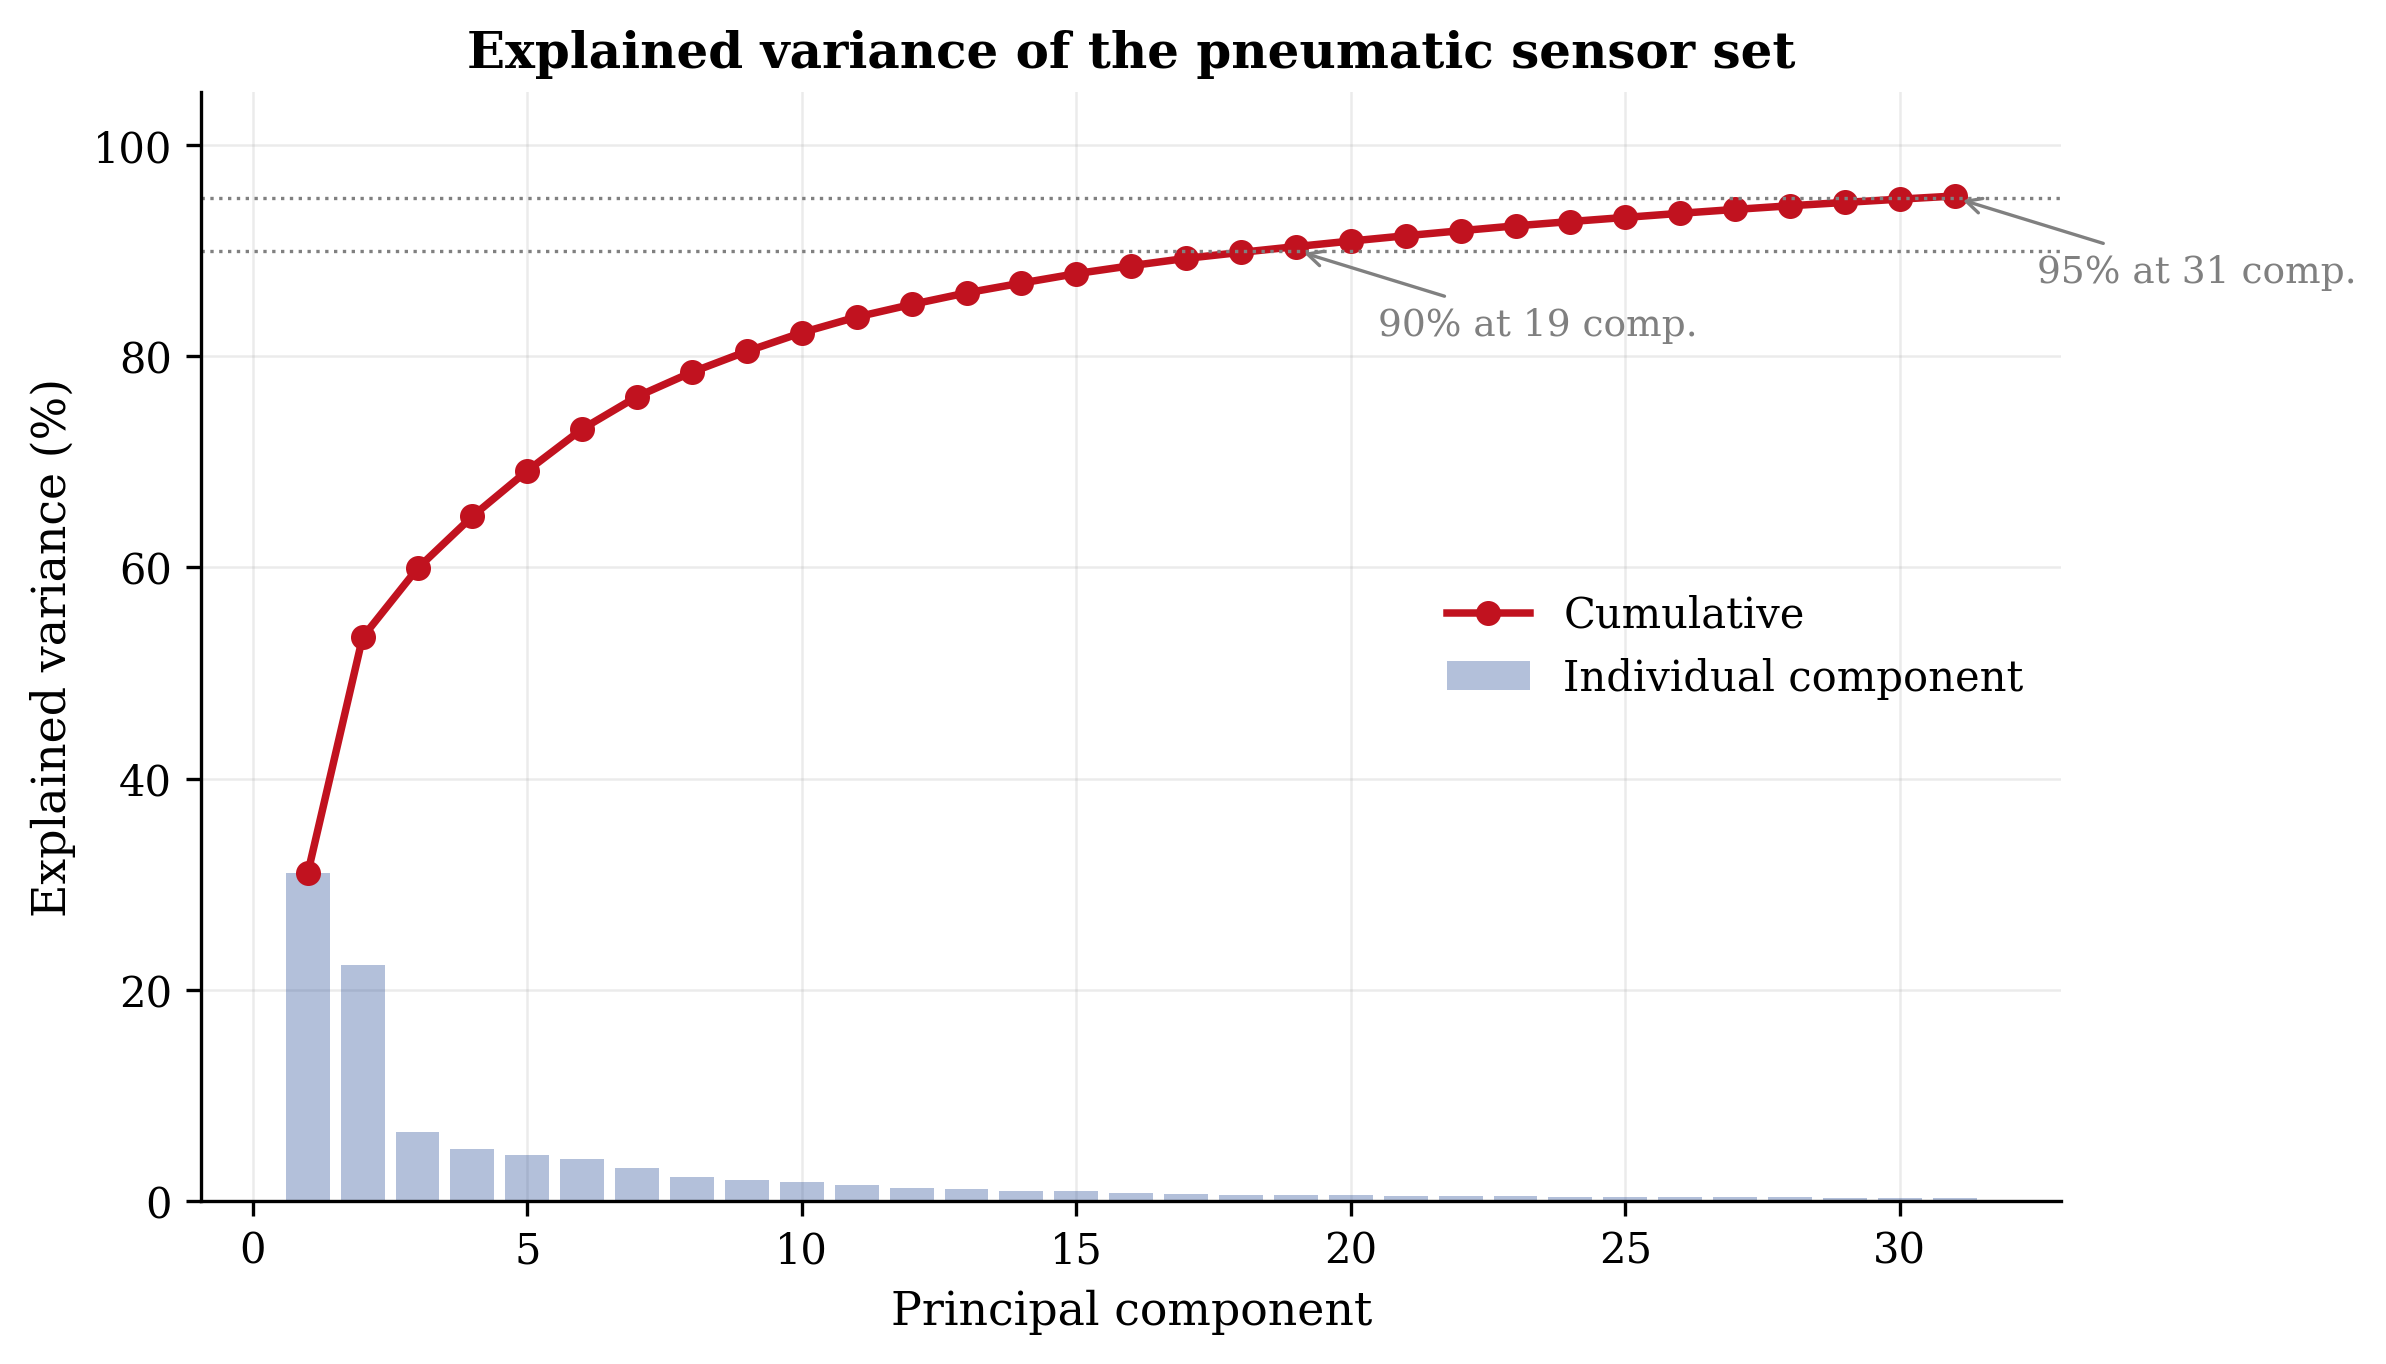
\includegraphics[width=0.8\linewidth]{pca_explained_variance.png}
  \caption{Cumulative explained variance of the pneumatic sensor set under PCA. Because 214
  sensor pairs are near-duplicates ($|r| > 0.98$) from per-wagon replication, a small number
  of components captures most of the variation, which is why the redundancy can be absorbed
  by PCA without dropping any columns.}
  \label{fig:pca}
\end{figure}
\chapter{Operational states}
\label{ch:states}

This chapter derives the operational regimes of the train and validates them. The regimes
are recovered by clustering, and, in line with the feature-role split
(Section~\ref{sec:roles}), they are defined from motion alone. Only the kinematic window
summaries (speed, acceleration, jerk, and their spreads) enter the clustering; the pneumatic
sensors are deliberately withheld so that they remain independent evidence in the chapters
that follow.

\section{Clustering into operational states}
\label{sec:kselection}

The states were obtained by k-means clustering of the motion window features, with the
number of clusters chosen by internal validation rather than fixed in advance. Two clustering
methods (k-means and hierarchical clustering on a sample) were run for $k$ from 2 to 6, and
four indicators were compared (Figure~\ref{fig:kselection}). The \emph{silhouette} score~\cite{Rousseeuw:87}
measures how well each window fits its own cluster relative to the nearest alternative; it
ranges over $[-1, 1]$, where values near 1 indicate well-separated clusters, values near 0 an
ambiguous assignment, and higher is better. The \emph{Davies--Bouldin} index~\cite{DaviesBouldin:79}
measures the average overlap between a cluster and its most similar neighbour; it is bounded
below by 0 and unbounded above, with lower values better. The \emph{Bayesian information
criterion} (BIC)~\cite{Schwarz:78} of a Gaussian mixture balances goodness of fit against model
complexity; it is not bounded to a fixed range and its absolute value is not interpretable, so
only differences between models are read, with lower values better. The \emph{adjusted Rand
index} (ARI) measures agreement between two clusterings; it takes the value 1 for identical
partitions and about 0 for the agreement expected by chance (it can be slightly negative), and
is used here both to compare the k-means and hierarchical labels and to assess stability under
resampling.

The per-$k$ values of all four indicators are collected in Table~\ref{tab:kselection}. The
silhouette score (Figure~\ref{fig:kselection}a) rises monotonically with $k$, from 0.48 at
$k=2$ to 0.60 at $k=6$, and the Davies--Bouldin index (Figure~\ref{fig:kselection}b) likewise
keeps improving as clusters are added, from 1.20 at $k=3$ to 0.95 at $k=6$. Both therefore
reward ever finer partitions and neither picks out a value on its own; this is the expected
behaviour of internal compactness indices, so the choice cannot rest on them alone. The two
clustering methods agree closely at both of the small $k$ that were cross-checked (cross-method
ARI 0.81 at $k=3$ and 0.77 at $k=4$), and the $k=4$ solution is stable under resampling
(bootstrap ARI about 0.87).

The BIC (Figure~\ref{fig:kselection}c) is informative for a specific reason: unlike the
silhouette and Davies--Bouldin scores it explicitly penalises model complexity, so rather than
improving without bound it is expected to flatten once additional clusters stop describing real
structure. Its absolute value is not meaningful; only the size of each successive drop is. The
largest single drop is the $k=3\rightarrow4$ step ($-121{,}900$), but the $k=4\rightarrow5$ step
is nearly as large ($-110{,}900$), so the BIC does not by itself separate four clusters from
five. What it does show is where the marginal gain collapses: the $k=5\rightarrow6$ step
($-54{,}000$) is less than half of either earlier step. The BIC therefore rules out large $k$
but leaves the choice between four and five to be settled on other grounds.

That choice is made on parsimony and physical interpretability. None of the internal indices
favours five clusters over four: the silhouette and Davies--Bouldin scores keep rising for any
$k$, and the BIC does not distinguish the two. The smaller model is therefore preferred unless
a fifth cluster earns its place with a distinct operating mode, and it does not. Four clusters
already exhaust the stop--accelerate--cruise--brake cycle of a metro duty cycle
(Table~\ref{tab:states}), each with its own signature in speed and the sign of acceleration,
whereas a fifth group adds no regime that is not already present. Four clusters is kept as the
most parsimonious description consistent with the metrics and with the physics of the duty
cycle.

\begin{table}[htbp]
  \centering
  \caption{Cluster-count selection metrics per $k$. Silhouette (higher better, range
  $[-1,1]$), Davies--Bouldin (lower better, $\geq 0$), cross-method ARI ($k$-means versus
  hierarchical; 1 is identical, computed for the two small $k$ that were cross-checked), and the
  Gaussian-mixture BIC (lower better; only differences are meaningful). $\Delta$BIC is the drop
  from the previous $k$. The largest drop is at $k=3\rightarrow4$, but $k=4\rightarrow5$ is
  comparable; the gain collapses only after $k=5$.}
  \label{tab:kselection}
  \begin{tabular}{rrrrrr}
    \toprule
    $k$ & Silhouette & Davies--Bouldin & Cross-method ARI & BIC ($\times 10^{3}$) & $\Delta$BIC ($\times 10^{3}$) \\
    \midrule
    2 & 0.476 & 0.999 & n/a  & $-999.1$  & n/a      \\
    3 & 0.535 & 1.196 & 0.81 & $-1088.8$ & $-89.8$  \\
    4 & 0.567 & 1.091 & 0.77 & $-1210.8$ & $-121.9$ \\
    5 & 0.587 & 0.990 & n/a  & $-1321.6$ & $-110.9$ \\
    6 & 0.605 & 0.945 & n/a  & $-1375.7$ & $-54.0$  \\
    \bottomrule
  \end{tabular}
\end{table}

\begin{figure}[htbp]
  \centering
  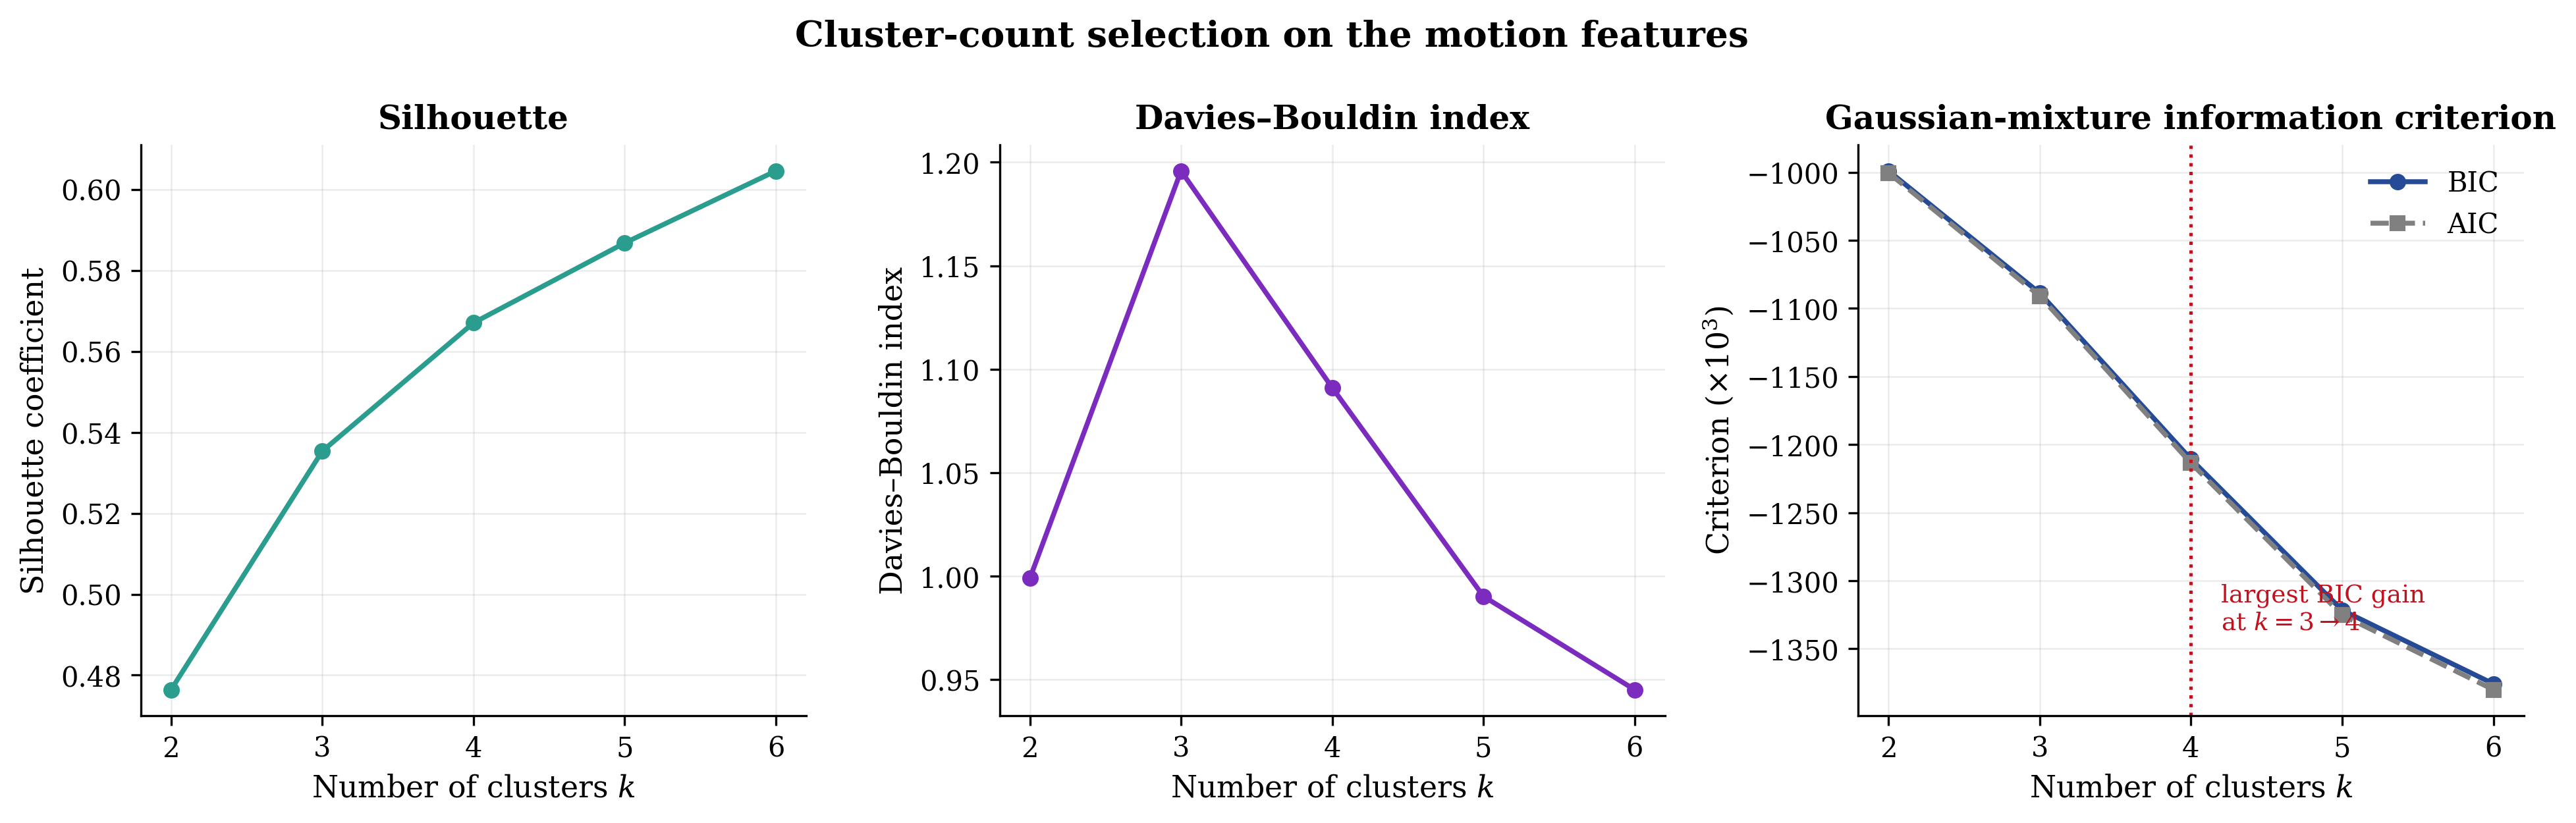
\includegraphics[width=0.9\linewidth]{kinematic_kselection.png}
  \caption{Cluster-count selection on the motion features. \textbf{(a)} Silhouette rises
  monotonically and \textbf{(b)} Davies--Bouldin keeps improving, so neither compactness index
  picks a $k$ on its own. \textbf{(c)} The Gaussian-mixture BIC has its largest drop at
  $k=3\rightarrow4$, but the $k=4\rightarrow5$ drop is comparable; the marginal gain collapses
  only after $k=5$. Four groups is retained on grounds of parsimony and physical
  interpretability (see text and Table~\ref{tab:kselection}).}
  \label{fig:kselection}
\end{figure}

\label{sec:fourstates}
Table~\ref{tab:states} numbers the four clusters and, for each, gives its held-out share, its
median motion, and the reasoning that maps it onto an operating regime. The regime labels used
in the rest of this report are read off from these medians rather than assigned in advance, so
that the naming follows from the data.

\begin{table}[htbp]
  \centering
  \caption{The four clusters on the held-out window, numbered in duty-cycle order. Shares and
  medians are computed on ten-second windows; velocity and acceleration are in normalised units.
  The final column states why each cluster's median motion identifies it with the named regime.}
  \label{tab:states}
  \begin{tabularx}{\linewidth}{c r r r >{\RaggedRight}X}
    \toprule
    Cluster & Median vel. & Median accel. & Share (\%) & Interpretation and justification \\
    \midrule
    1 & 0.000 & \phantom{$-$}0.000 & 48.12 & Zero speed and zero acceleration: the train is at
        rest, labelled \emph{standing}. \\[0.4ex]
    2 & 0.305 & \phantom{$-$}0.041 & 14.34 & Moderate speed with the largest positive median
        acceleration: the train is speeding up, labelled \emph{accelerating}. \\[0.4ex]
    3 & 0.842 & \phantom{$-$}0.002 & 17.27 & Highest median speed with near-zero acceleration:
        steady running, labelled \emph{cruising}. \\[0.4ex]
    4 & 0.343 & $-$0.033 & 20.26 & Moderate speed with clearly negative acceleration: the train
        is slowing down, labelled \emph{deceleration}. \\
    \bottomrule
  \end{tabularx}
\end{table}

The resulting profile matches a typical metro duty cycle. Standing dominates at about 48\% of
windows, with zero median speed and acceleration. Cruising has the highest median speed
(0.84) and near-zero acceleration. Accelerating and deceleration sit at intermediate speeds
and are separated by the sign of acceleration ($+0.041$ against $-0.033$). Deceleration
accounts for about one window in five (20.3\%), which sets the scale for the braking analysis
in Chapter~\ref{ch:braking}. Figure~\ref{fig:profiles} shows the four motion profiles, and
Figure~\ref{fig:velaccel} the velocity--acceleration cycle the train traces through them.

\begin{figure}[htbp]
  \centering
  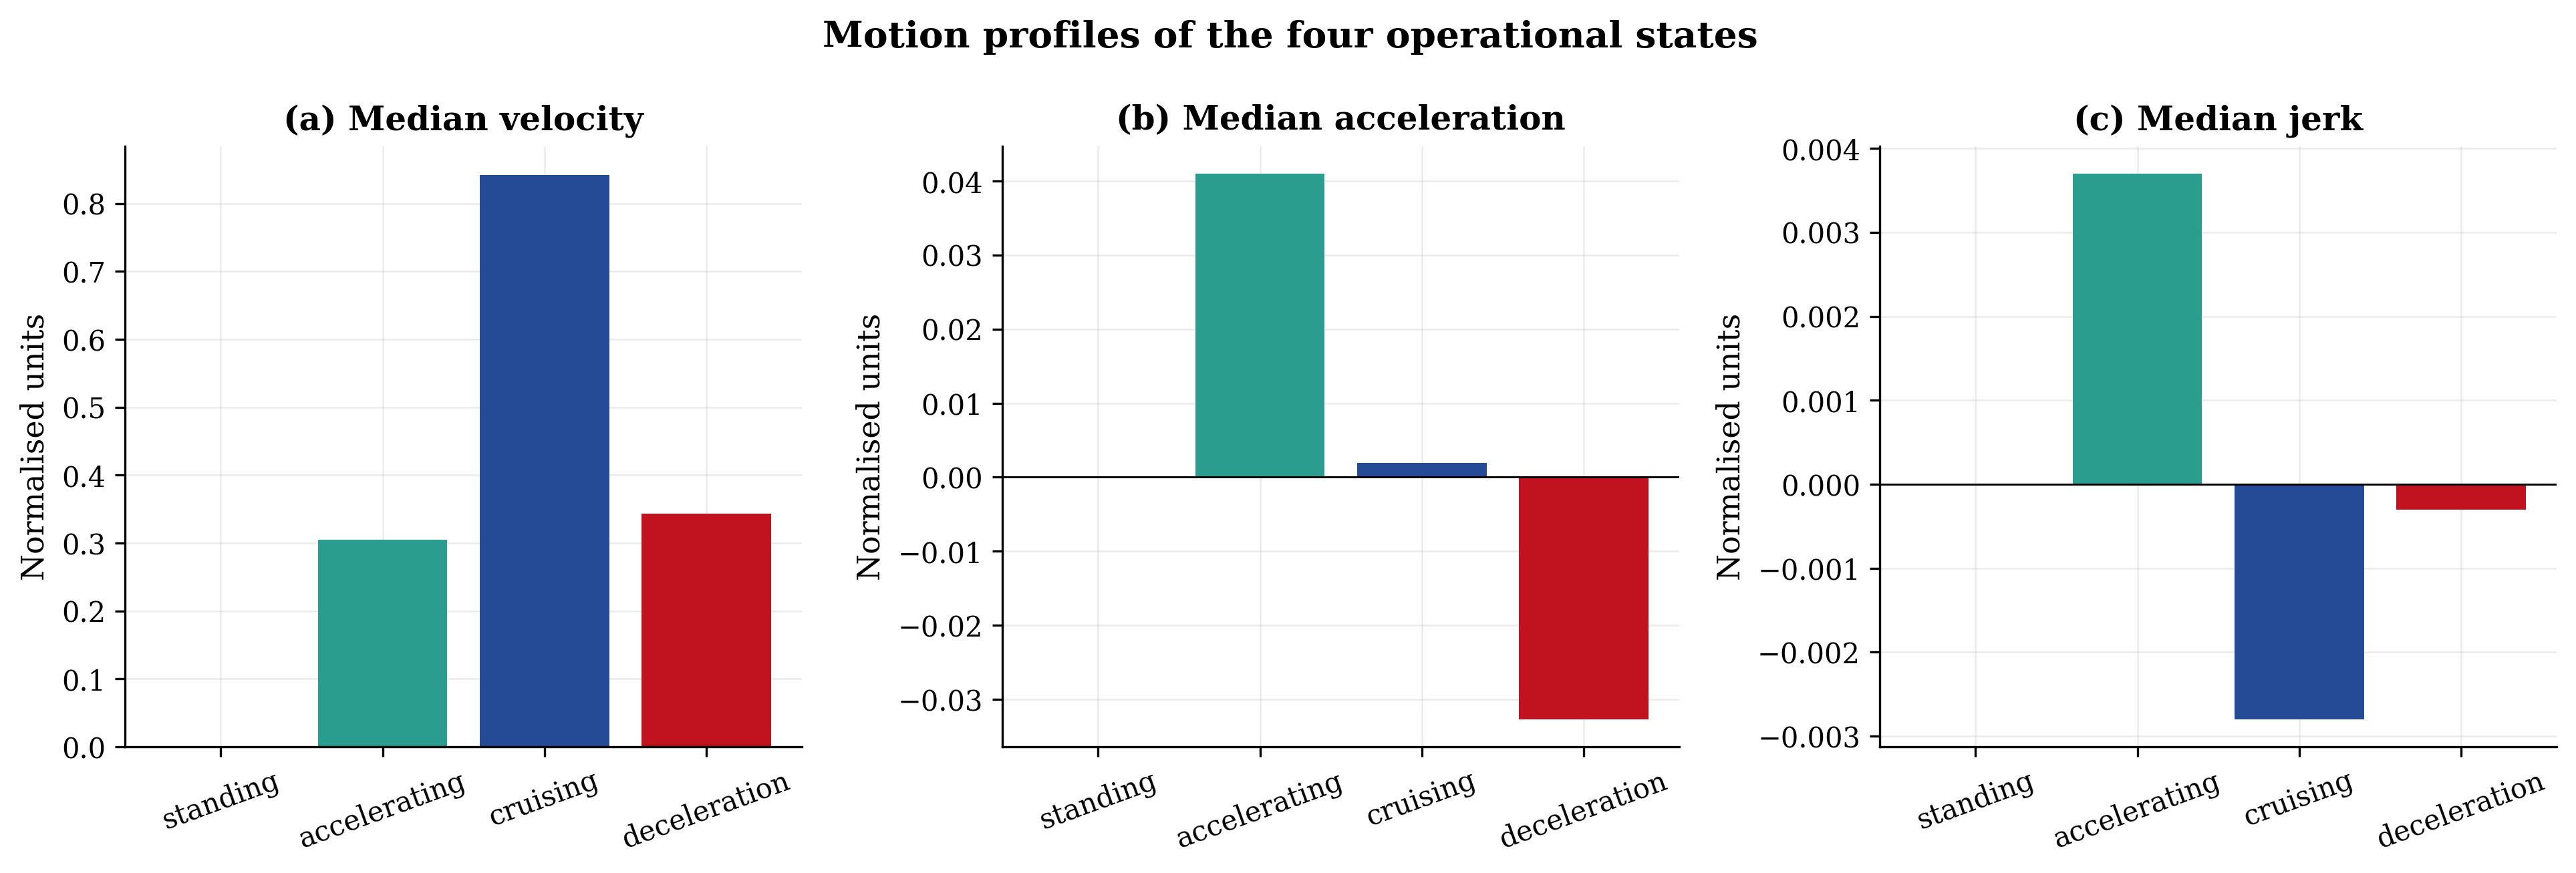
\includegraphics[width=0.9\linewidth]{state_profiles.png}
  \caption{Motion profiles of the four states: \textbf{(a)} median velocity, \textbf{(b)} median
  acceleration, and \textbf{(c)} median jerk. The states are separated by speed and the sign and
  magnitude of acceleration; no pneumatic channel enters the definition.}
  \label{fig:profiles}
\end{figure}

\begin{figure}[htbp]
  \centering
  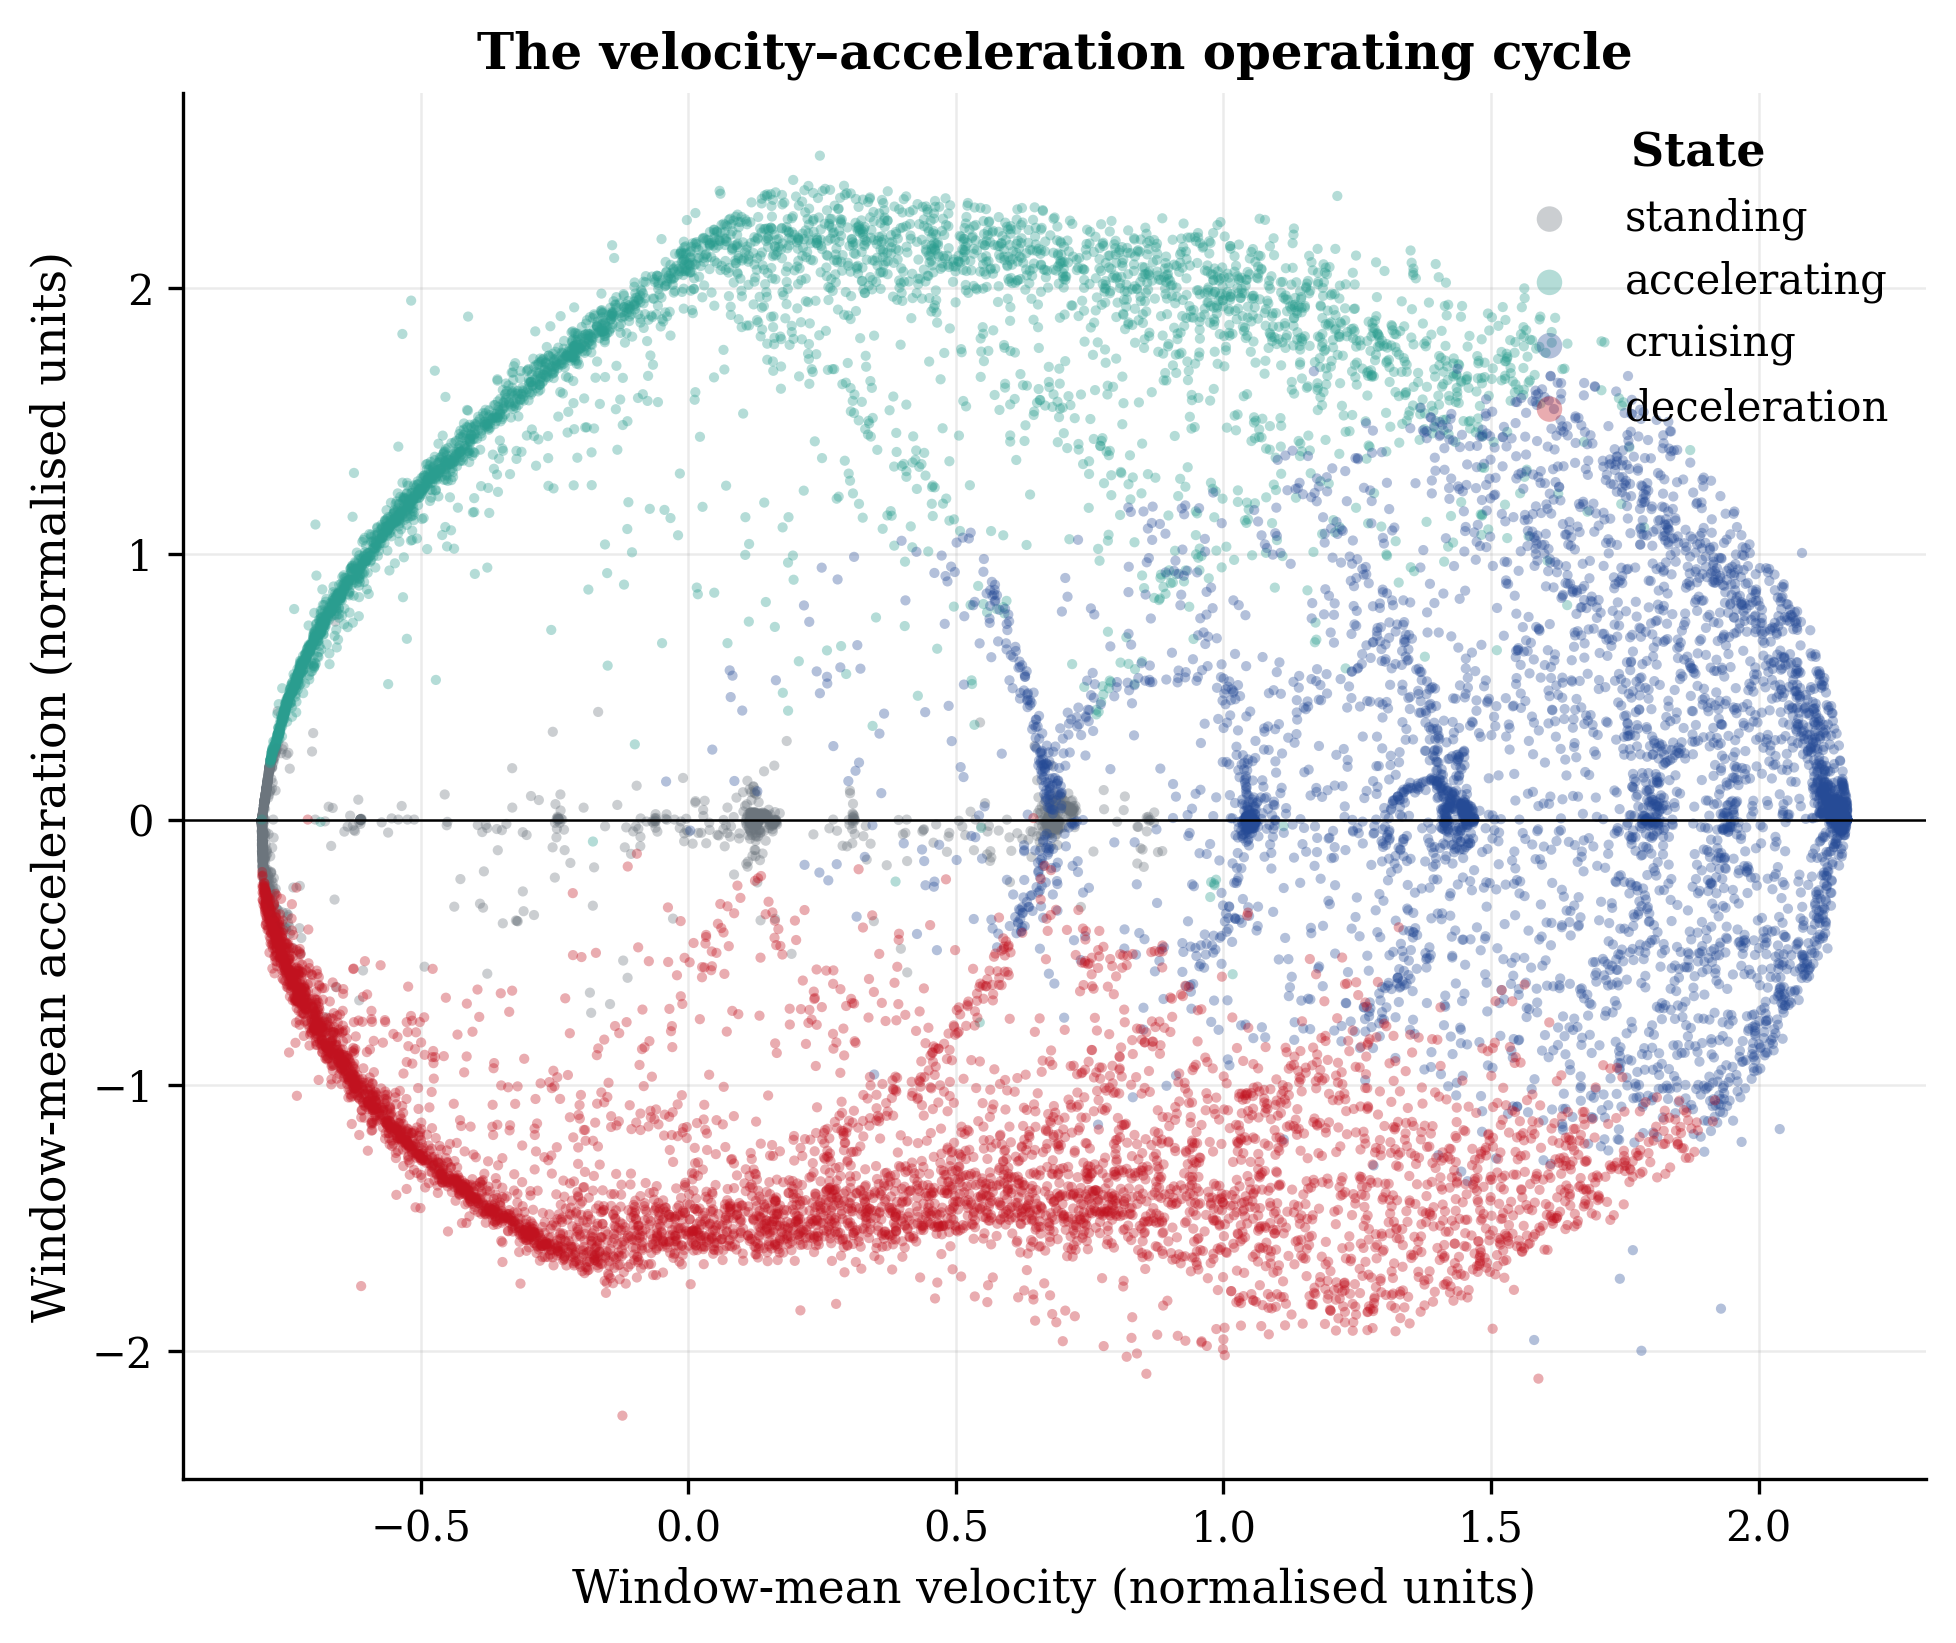
\includegraphics[width=0.75\linewidth]{kinematic_vel_accel_scatter.png}
  \caption{The velocity--acceleration cycle, coloured by state. The train moves anticlockwise:
  stop, accelerate, cruise, decelerate, stop. A minority of off-curve points do not fit the
  idealised cycle and motivate future work (Chapter~\ref{ch:conclusion}).}
  \label{fig:velaccel}
\end{figure}

\section{Plausibility of four states}
\label{sec:heldbrake}

An earlier version of this analysis included brake-pressure sensors in the state definition.
It systematically mislabelled a stationary train holding its brake at a station as
deceleration: the brake was applied, so the pneumatic signal resembled braking even though
the train was not moving. This is precisely the circularity that the feature-role split
(Section~\ref{sec:roles}) is designed to avoid, and it is the reason the state definition was
restricted to motion. Table~\ref{tab:heldbrake} shows how the earlier, pneumatics-contaminated
\enquote{braking} label redistributes under the motion-only definition. Of the windows the
old label called braking, about 105{,}000 are genuine deceleration, roughly 80{,}000 are in
fact acceleration, and about 47{,}000 are a stationary train holding its brake. Rather than discarding this information whether a standing train is braked is retained as a sub-label
(\texttt{standing\_braked} versus \texttt{standing\_idle}), but it no longer contaminates the
deceleration regime, which is 99.9\% genuine deceleration under the corrected definition.

\begin{table}[htbp]
  \centering
  \caption{Reassignment of the old, pneumatics-contaminated \enquote{braking} label under the
  motion-only definition. Windows counted at the window level.}
  \label{tab:heldbrake}
  \begin{tabular}{lr}
    \toprule
    Motion-only state & Windows from old \enquote{braking} \\
    \midrule
    accelerating & 80{,}226 \\
    deceleration & 104{,}908 \\
    cruising     & 519 \\
    standing     & 46{,}723 \\
    \bottomrule
  \end{tabular}
\end{table}

As a second check, the motion-only clustering was compared against a classifier trained on
the full feature set. A Random Forest predicting the state labels from both the kinematic and
the pneumatic window summaries reaches 0.994 accuracy on held-out windows, and its most
important features are the kinematic ones: the mean, maximum, and minimum of acceleration,
and the mean and spread of speed. Pneumatic channels appear only much lower in the ranking.
Even when the pneumatic signals are made available, then, the states remain separable by
motion alone, which confirms that they are motion-defined regimes rather than an artefact of
the pneumatic data.

\section{Transitions and dwell}

The states occur in the expected order (stop, accelerate, cruise, brake, stop), and the
transition matrix is dominated by this cycle (Figure~\ref{fig:transitions}). Mean dwell times
match the physical picture: standing about 54\,s (with very high variance, since layovers and
terminus stops are long and irregular), accelerating about 17\,s, cruising about 21\,s, and
deceleration about 24\,s. The state mix is stable from month to month
(Figure~\ref{fig:bymonth}), which indicates that the regimes are a property of how the train
is operated rather than of any particular period in the recording.

\begin{figure}[htbp]
  \centering
  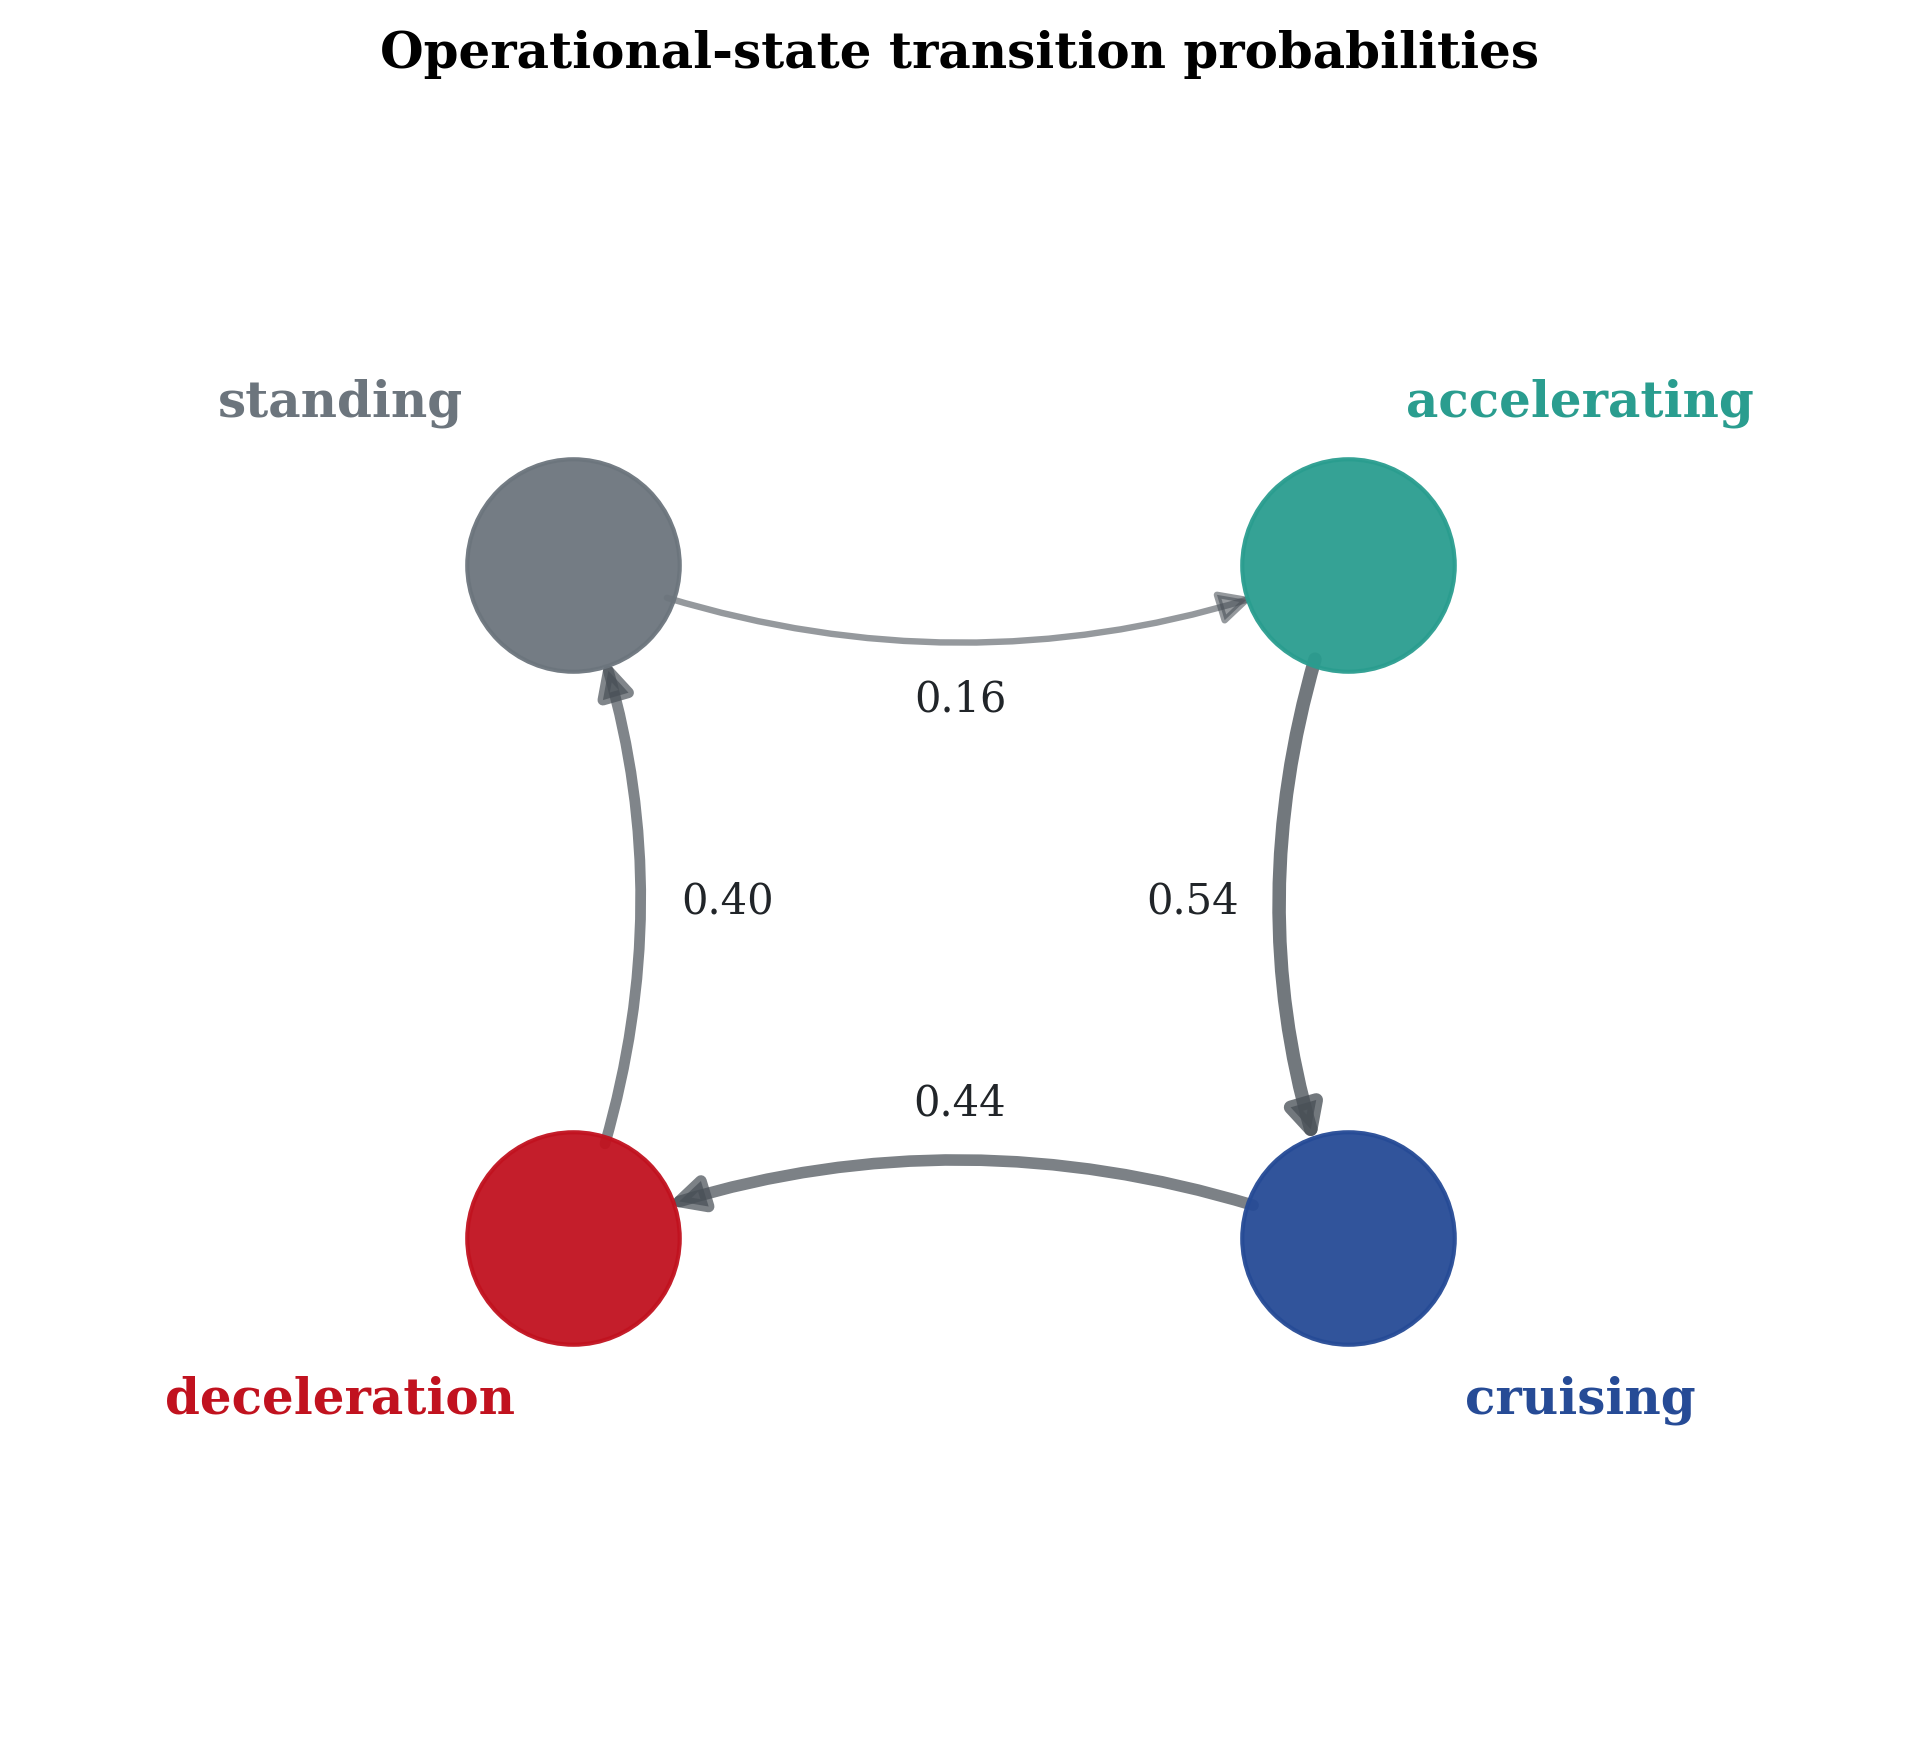
\includegraphics[width=0.7\linewidth]{transition_diagram.png}
  \caption{State transition diagram. The dominant path is the operating cycle
  stop\,$\rightarrow$\,accelerate\,$\rightarrow$\,cruise\,$\rightarrow$\,decelerate\,$\rightarrow$\,stop.}
  \label{fig:transitions}
\end{figure}

\begin{figure}[htbp]
  \centering
  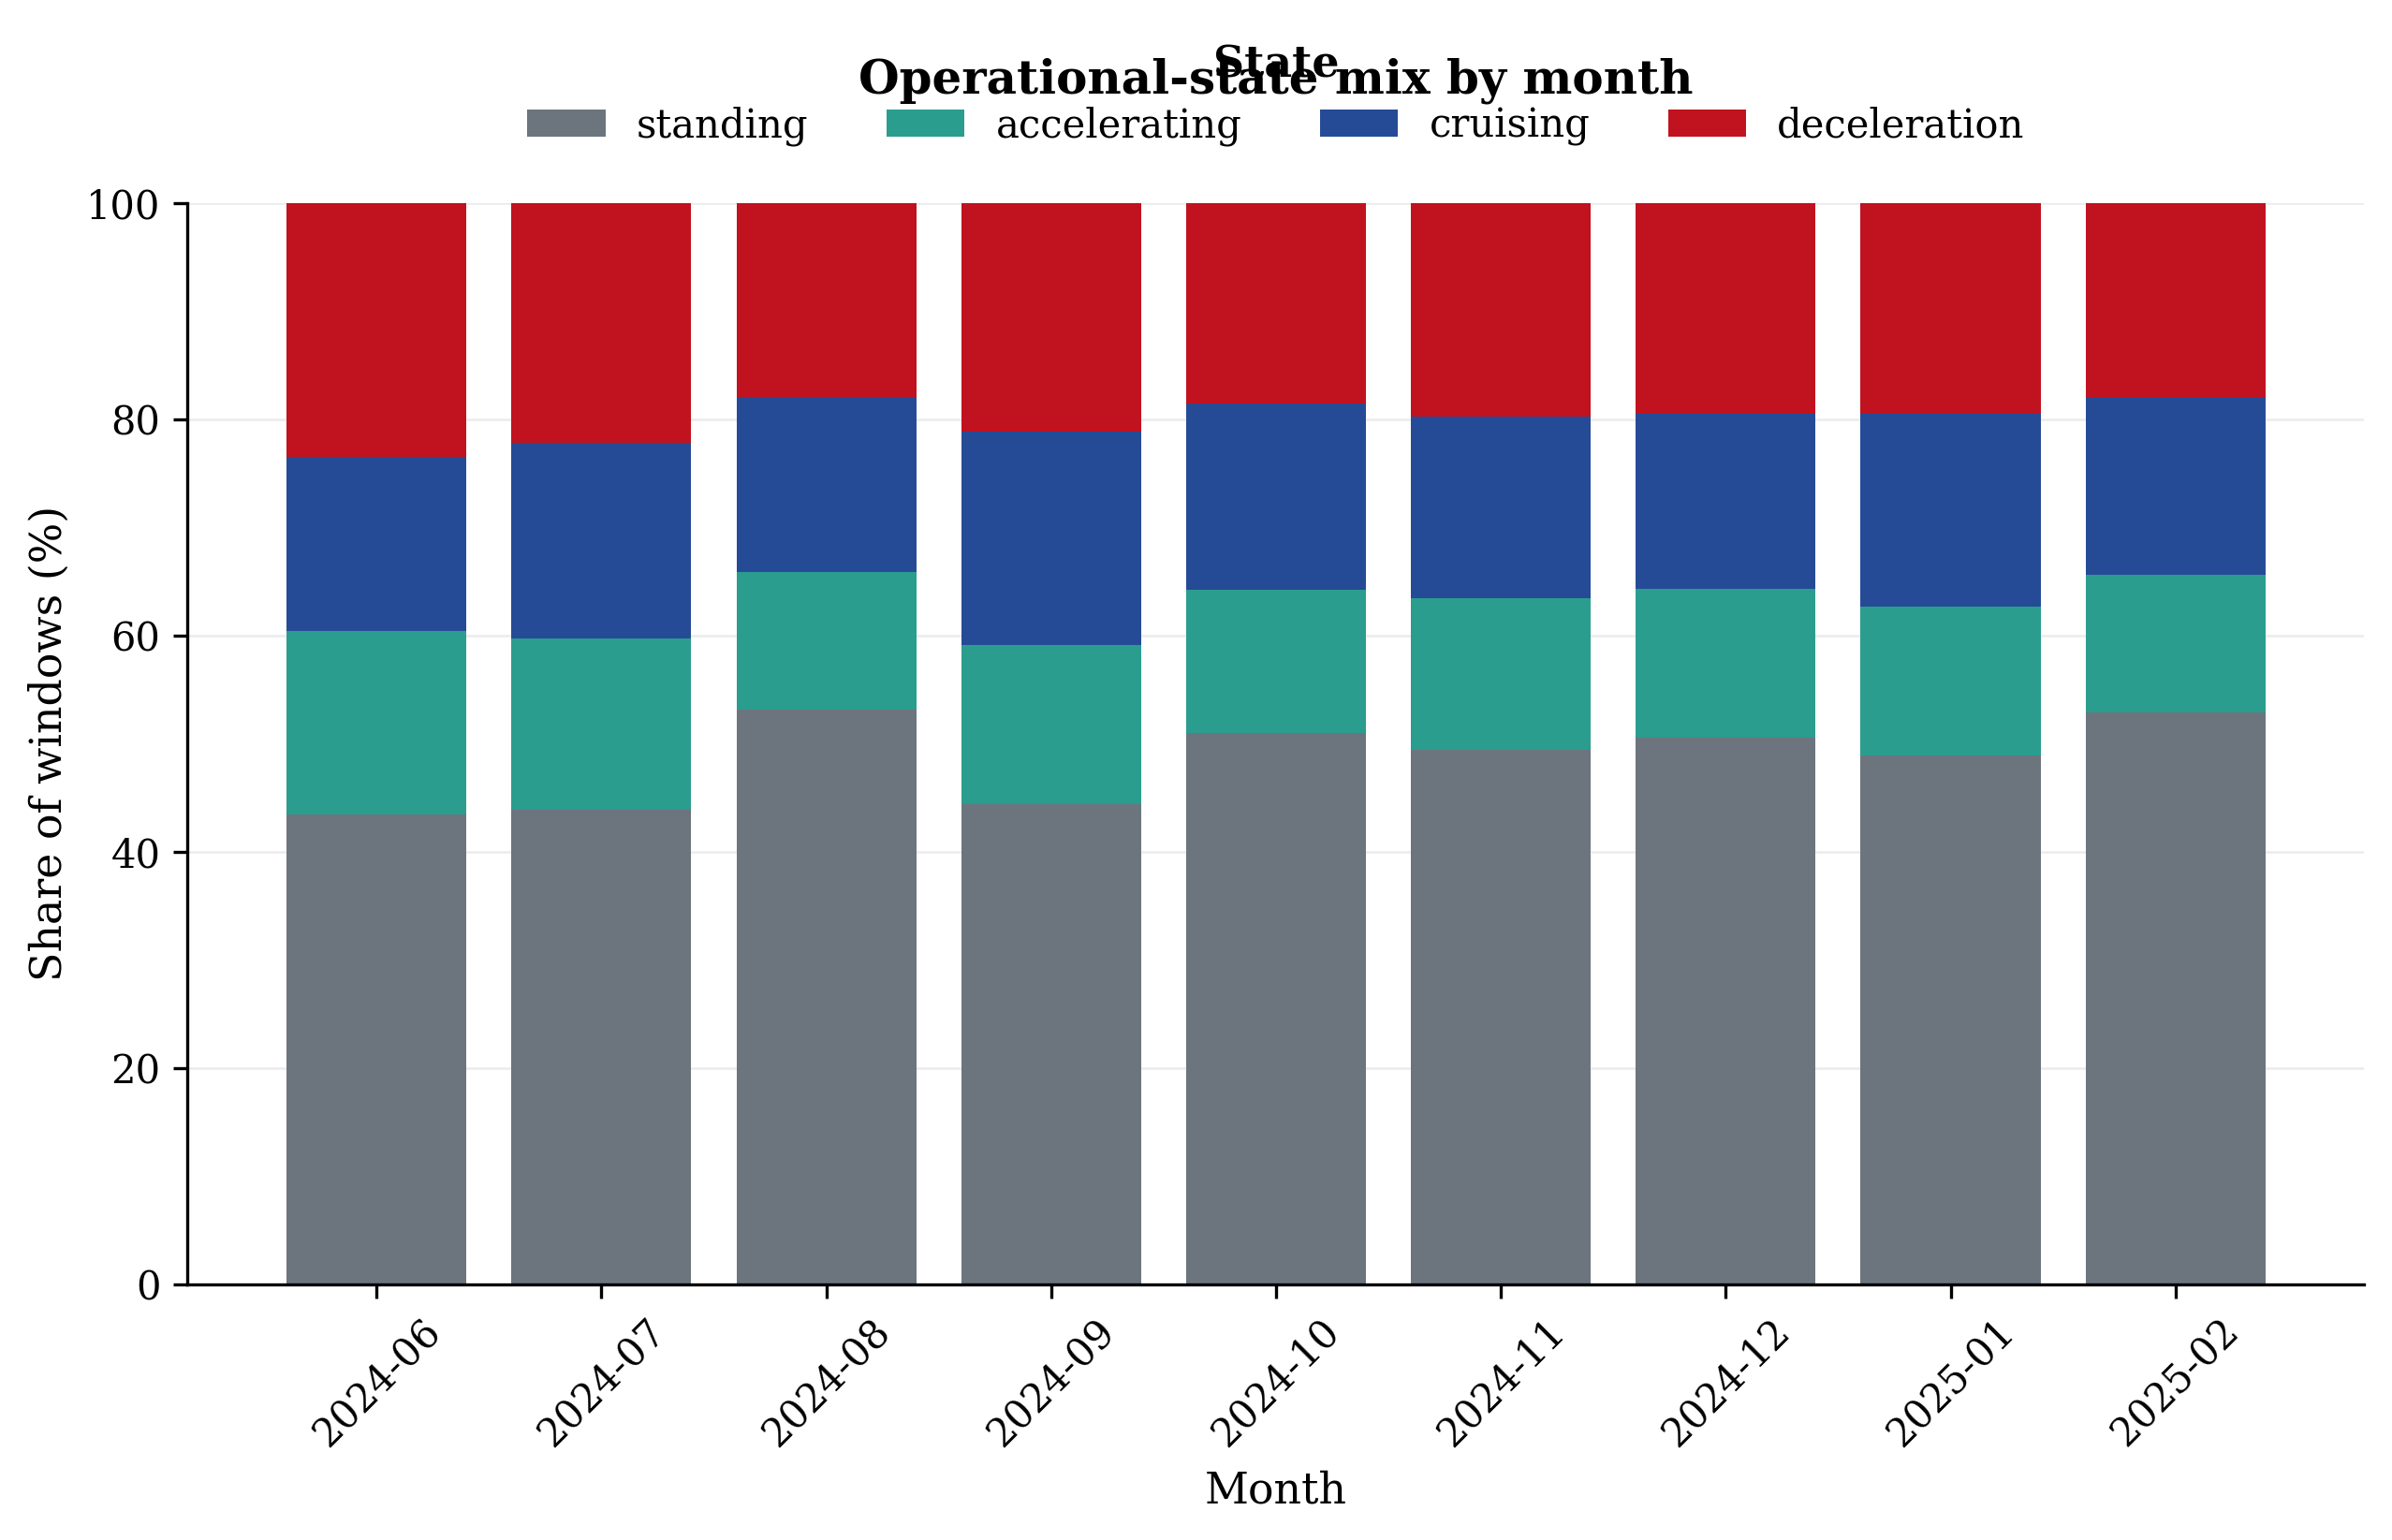
\includegraphics[width=0.9\linewidth]{state_distribution_by_month.png}
  \caption{State mix by month. The proportions are stable across the recording, so the regimes
  reflect the operating pattern rather than a seasonal artefact.}
  \label{fig:bymonth}
\end{figure}

\section{Robustness to window length}
\label{sec:window-sensitivity}

Because the ten-second window is a design choice, the clustering was re-run at 5, 10, 15, and
20 seconds as a read-only sensitivity check that left the canonical ten-second models
untouched (Figure~\ref{fig:windowsens}). The deceleration share is essentially flat across
all four sizes, about 20\% at each. The state \emph{chatter} rate, the fraction of windows
whose state differs from an adjacent window, rises with window length, from about 0.19 at
5\,s to 0.54 at 20\,s. Short windows are therefore not the source of label churn, and ten
seconds is a sensible compromise between resolution and stability.

\begin{figure}[htbp]
  \centering
  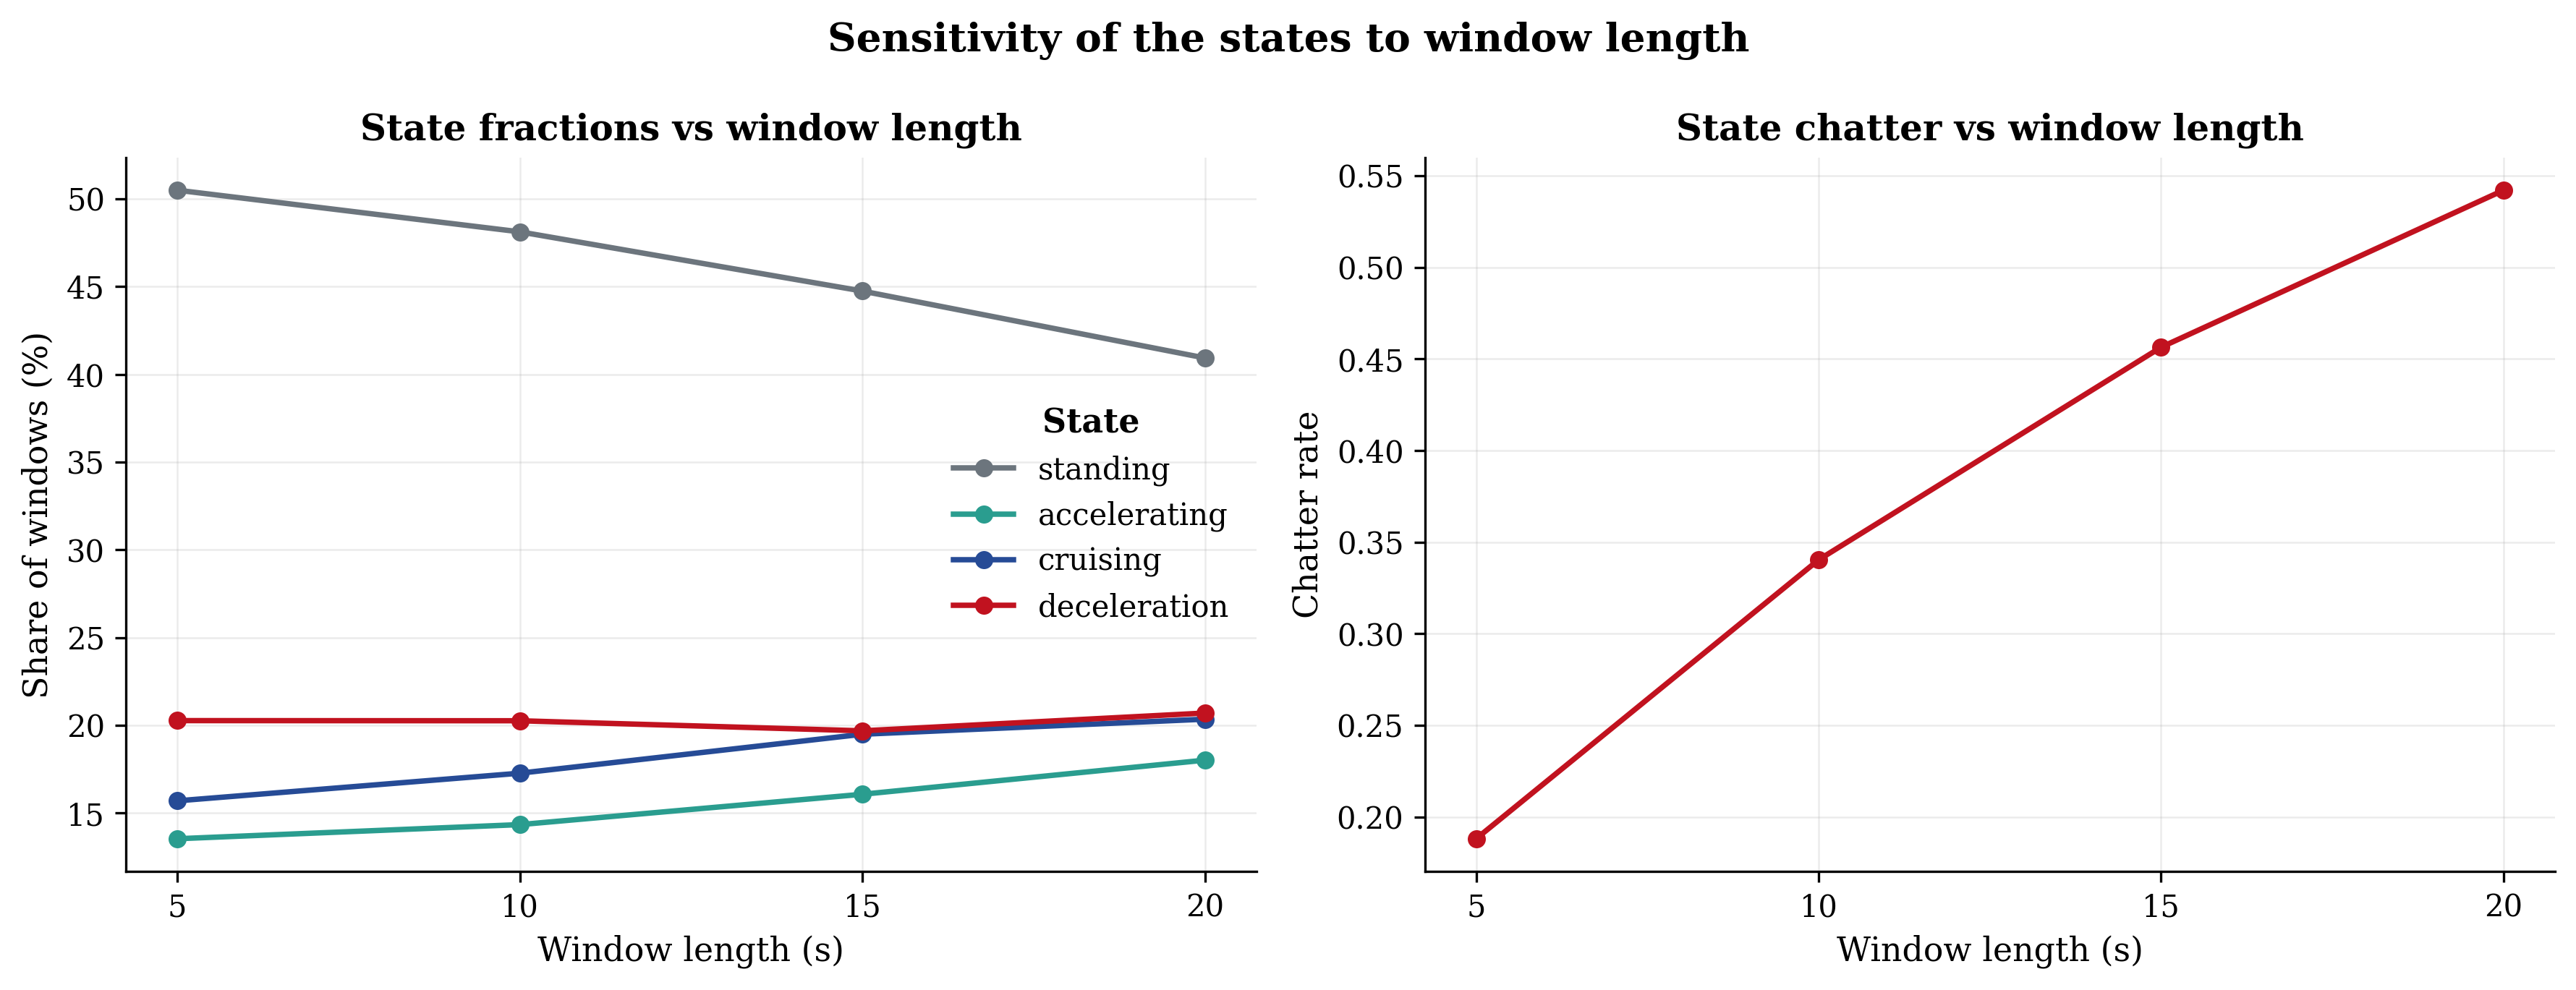
\includegraphics[width=0.9\linewidth]{window_sensitivity.png}
  \caption{Window-length sensitivity. State fractions (left) are stable across 5--20\,s; the
  deceleration share stays near 20\%. Chatter (right) rises with window length, so short
  windows are not the cause of label churn.}
  \label{fig:windowsens}
\end{figure}

\section{Pre-event state distribution}
\label{sec:preevent}

As an initial link to the maintenance record, the mix of operational states in the 24 to
72~hours before each documented failure or maintenance event was compared with the overall
baseline. Across 62 event-by-window-size chi-square tests, 61 were significant at $p<0.05$.
This significance is, however, an artefact of sample size: with 6{,}000 to 24{,}000 windows
per test, even negligible differences reach significance. The effect size is small
throughout: Cramér's $V$ does not exceed 0.07 and is typically about 0.018, an order of
magnitude below the 0.1 value conventionally regarded as small.

The shift that does exist reflects the train standing idle in the depot before scheduled work.
Ahead of planned revisions the standing fraction rises by roughly 45 to 52 percentage points.
Restricting the test to moving windows, by dropping the standing state, reduces the effect
size roughly sixfold, to a Cramér's $V$ of about 0.003, which is indistinguishable from zero.
For the eight brake failures specifically there is no such idling, since failures occur in
service, and no meaningful effect size either.

The test therefore confirms only that the pipeline registers when the train is parked before
scheduled maintenance, which is an operational sanity check rather than evidence that
pre-failure braking behaviour differs from normal operation. This is consistent with the
near-null pre-failure braking signal reported in Chapter~\ref{ch:failure}, and it motivates
examining charging and idle windows with the auxiliary sensors, rather than deceleration, in
future work.
\chapter{Classification}
\label{ch:classification}

The operational states of Chapter~\ref{ch:states} were defined from motion alone. This
chapter asks the leakage-free question that motivates the whole design: can the
\emph{air-system} sensors, which never touched that definition, recover the deceleration
state on their own? If they can, deceleration leaves an independent fingerprint across the
pneumatic system, which is the premise the later analysis rests on.

\section{Setup}

The target is the binary label \enquote{deceleration versus not} on ten-second windows.
The motion channels that defined the target are excluded from the predictors entirely, in
line with the role ledger (Section~\ref{sec:roles}). Two predictor tiers are compared:

\begin{itemize}
  \item \textbf{auxiliary only} (60 features): the channels classed \emph{auxiliary} in the
        role ledger (Section~\ref{sec:roles}): the health and support channels (main-reservoir
        and load pressure, load signal, energy-braking resistance, ambient temperature, and
        compressor state). They are termed auxiliary because they never carry the brake command:
        they report the state of the air system rather than the braking demand itself, so
        recovering deceleration from them alone is the strictest test of independent signal.
  \item \textbf{full} (180 features): the auxiliary channels together with the \emph{actuation}
        channels (the brake command and its immediate pneumatic response), which, unlike the
        auxiliary channels, are driven directly by the braking demand.
\end{itemize}

Several transparent models are fitted so that the result does not hinge on one method's
quirks: a decision tree, LDA, QDA, logistic regression, and a random forest. All are
trained on the training window and scored on the held-out window
(Section~\ref{sec:split}). Because deceleration is the minority class (about 20\% of
windows), balanced accuracy and ROC-AUC are read in preference to raw accuracy.

\section{Results}

The headline numbers are in Table~\ref{tab:clf}. The full-tier random forest reaches a
ROC-AUC of 0.954 on held-out data, with balanced accuracy 0.869 and recall 0.956 for the
deceleration class. Its precision is lower, 0.528: the model catches almost all
decelerations but also flags a fair number of non-decelerations, which is the expected
trade-off when recall is high on a minority class and is the reason balanced accuracy and
AUC are the yardsticks here rather than precision alone. LDA and the decision tree follow
closely (AUC 0.924 and 0.910); the decision tree is the simplest model yet lands near the
top, making it the most interpretable strong option. QDA reaches 0.901 and logistic
regression 0.908. Full per-model metrics for both tiers are collected in
Appendix~\ref{app:clfmetrics}.

The auxiliary-only tier result is the most interesting. With the brake command \emph{withheld}, the
random forest still reaches AUC 0.921. Deceleration therefore leaves a fingerprint across
the independent health sensors (reservoir pressure, load pressure, and the rest) even
without being told the brake was applied. Most of the recoverable signal lives in the
auxiliary channels, not only in the actuation channels, which is what makes the pneumatic
system a plausible place to look for wear.

\subsection*{Which channels carry the signal}
\label{sec:clf-importance}

The interpretable models agree on where the deceleration signal sits. The decision tree
puts almost all of its weight on a single channel, pneumatic braking force, with spring-brake
pressure and proportional-valve pressure filling in the lower splits
(Table~\ref{tab:clfimp}). LDA spreads its weight more evenly but ranks the same subsystem
first: the per-wagon pneumatic-braking-force and proportional-valve-pressure copies dominate
its discriminant, with reservoir pressure the strongest auxiliary contributor. QDA exposes
no single loading vector, but it reaches comparable AUC on the same channel pool, so all
three lean on the same part of the pneumatic system. The channels that matter are the ones
that actuate and support braking, and none of them entered the motion-only state definition.

\begin{table}[htbp]
  \centering
  \caption{Top air-system channels for the full-tier classifiers. The decision-tree column
  is the split importance; the LDA column is the standardised discriminant weight
  ($|\text{coef}|$). Per-wagon copies are collapsed to their channel family.}
  \label{tab:clfimp}
  \begin{tabular}{lrr}
    \toprule
    Channel (family) & Decision tree & LDA $|\text{coef}|$ \\
    \midrule
    pneumatic braking force        & 0.69 & high \\
    spring-brake pressure          & 0.14 & low \\
    proportional-valve pressure    & 0.11 & highest \\
    energy-braking resistance      & 0.05 & low \\
    main-reservoir pressure        & 0.00 & moderate \\
    \bottomrule
  \end{tabular}
\end{table}

\begin{table}[htbp]
  \centering
  \caption{Deceleration classification on the held-out window. The full-tier random forest
  leads; the auxiliary-only random forest, with the brake command withheld, is nearly as
  strong. AUC is measured against 0.5 (coin flip); balanced accuracy against per-class
  chance.}
  \label{tab:clf}
  \begin{tabular}{llrrr}
    \toprule
    Tier & Model & ROC-AUC & Balanced acc. & $F_1$ (decel.) \\
    \midrule
    full          & random forest & 0.954 & 0.869 & 0.680 \\
    full          & LDA           & 0.924 & 0.726 & 0.610 \\
    full          & decision tree & 0.910 & 0.825 & 0.609 \\
    full          & QDA           & 0.901 & 0.746 & 0.602 \\
    auxiliary only & random forest & 0.921 & 0.831 & 0.620 \\
    \bottomrule
  \end{tabular}
\end{table}

\begin{figure}[htbp]
  \centering
  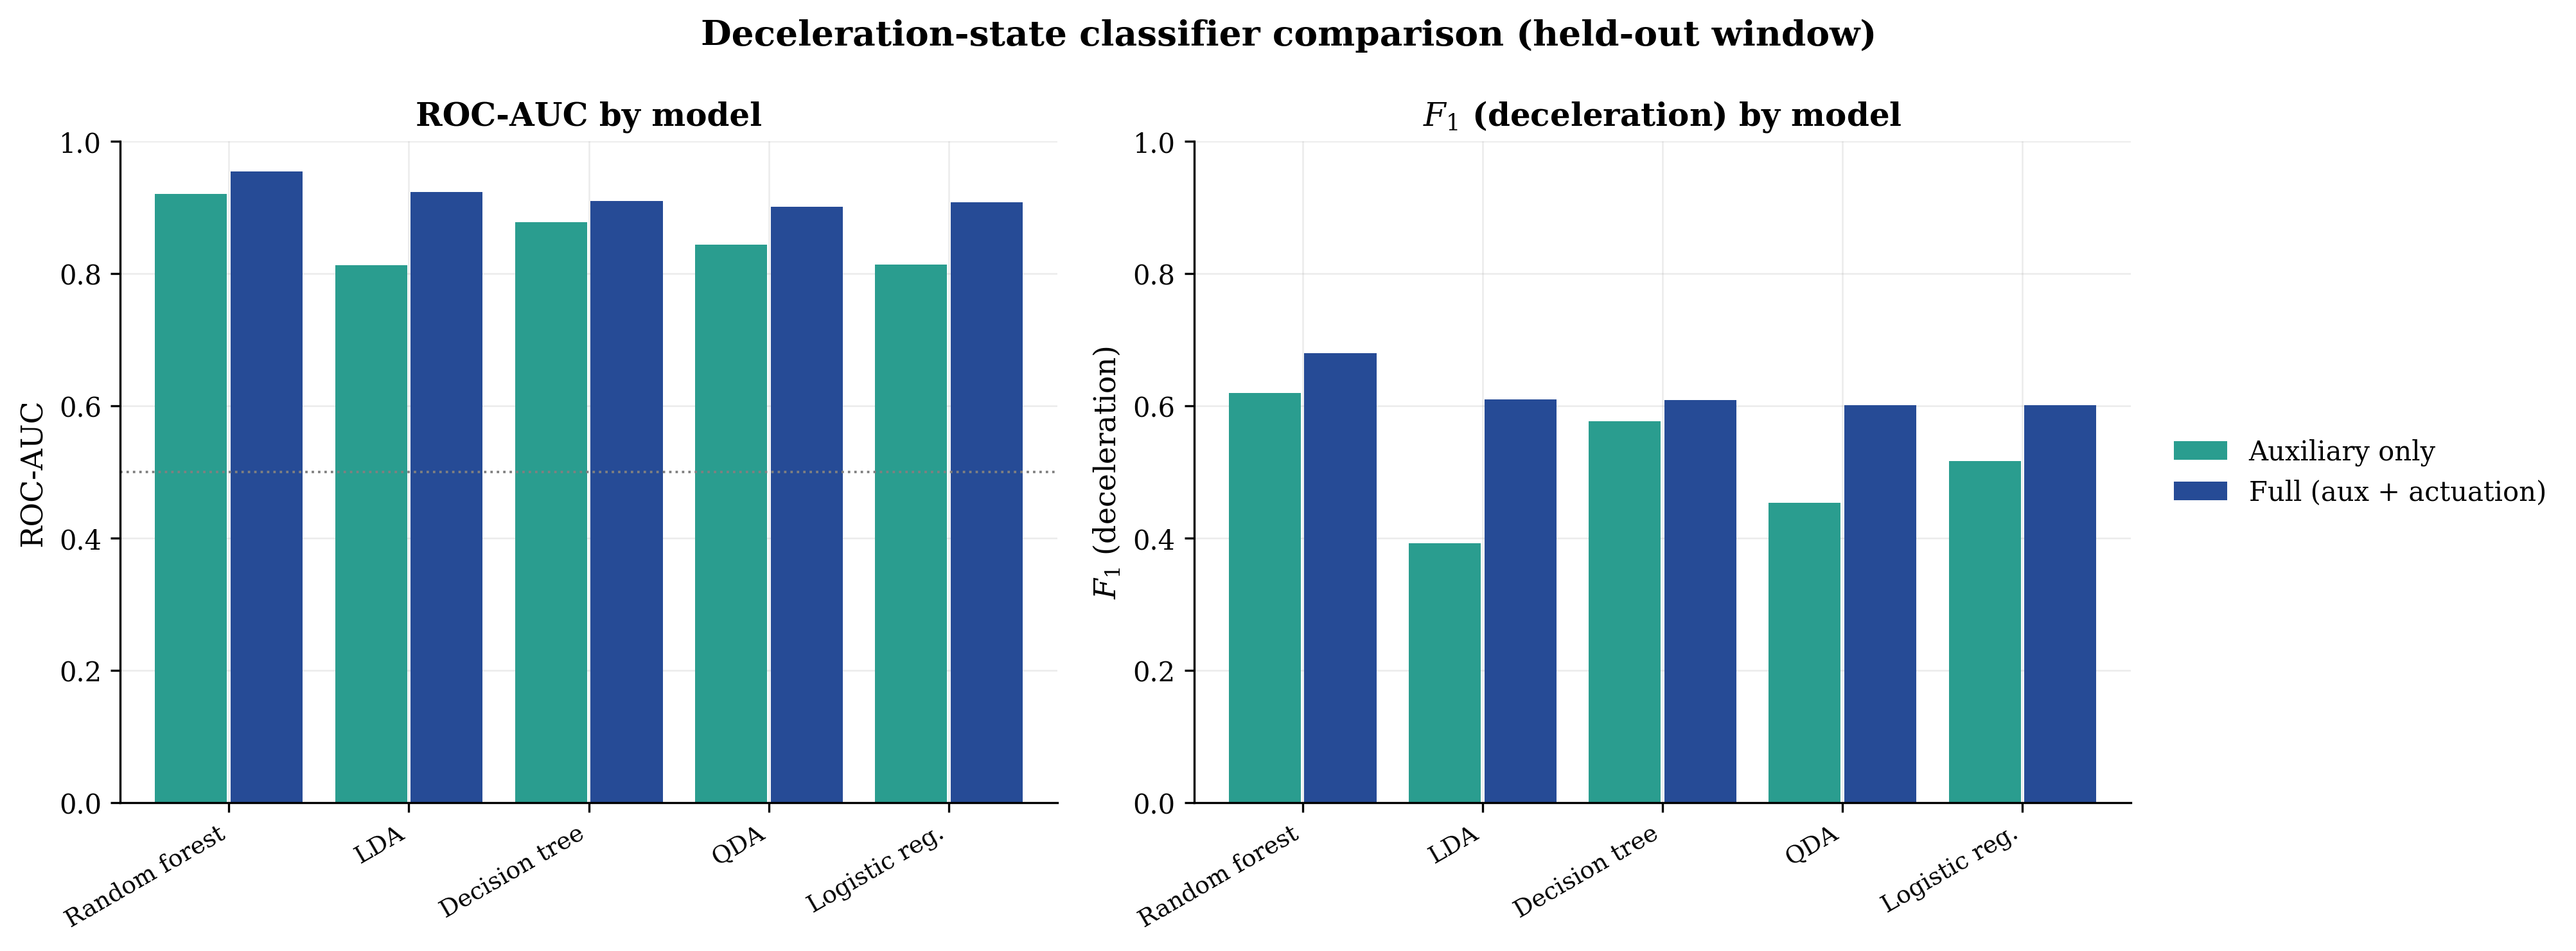
\includegraphics[width=0.9\linewidth]{state_clf_comparison.png}
  \caption{Model comparison for deceleration recovery (held-out AUC and $F_1$). The
  full-tier random forest leads; the auxiliary-only tier, without the brake command,
  remains close.}
  \label{fig:clfcomparison}
\end{figure}

\begin{figure}[htbp]
  \centering
  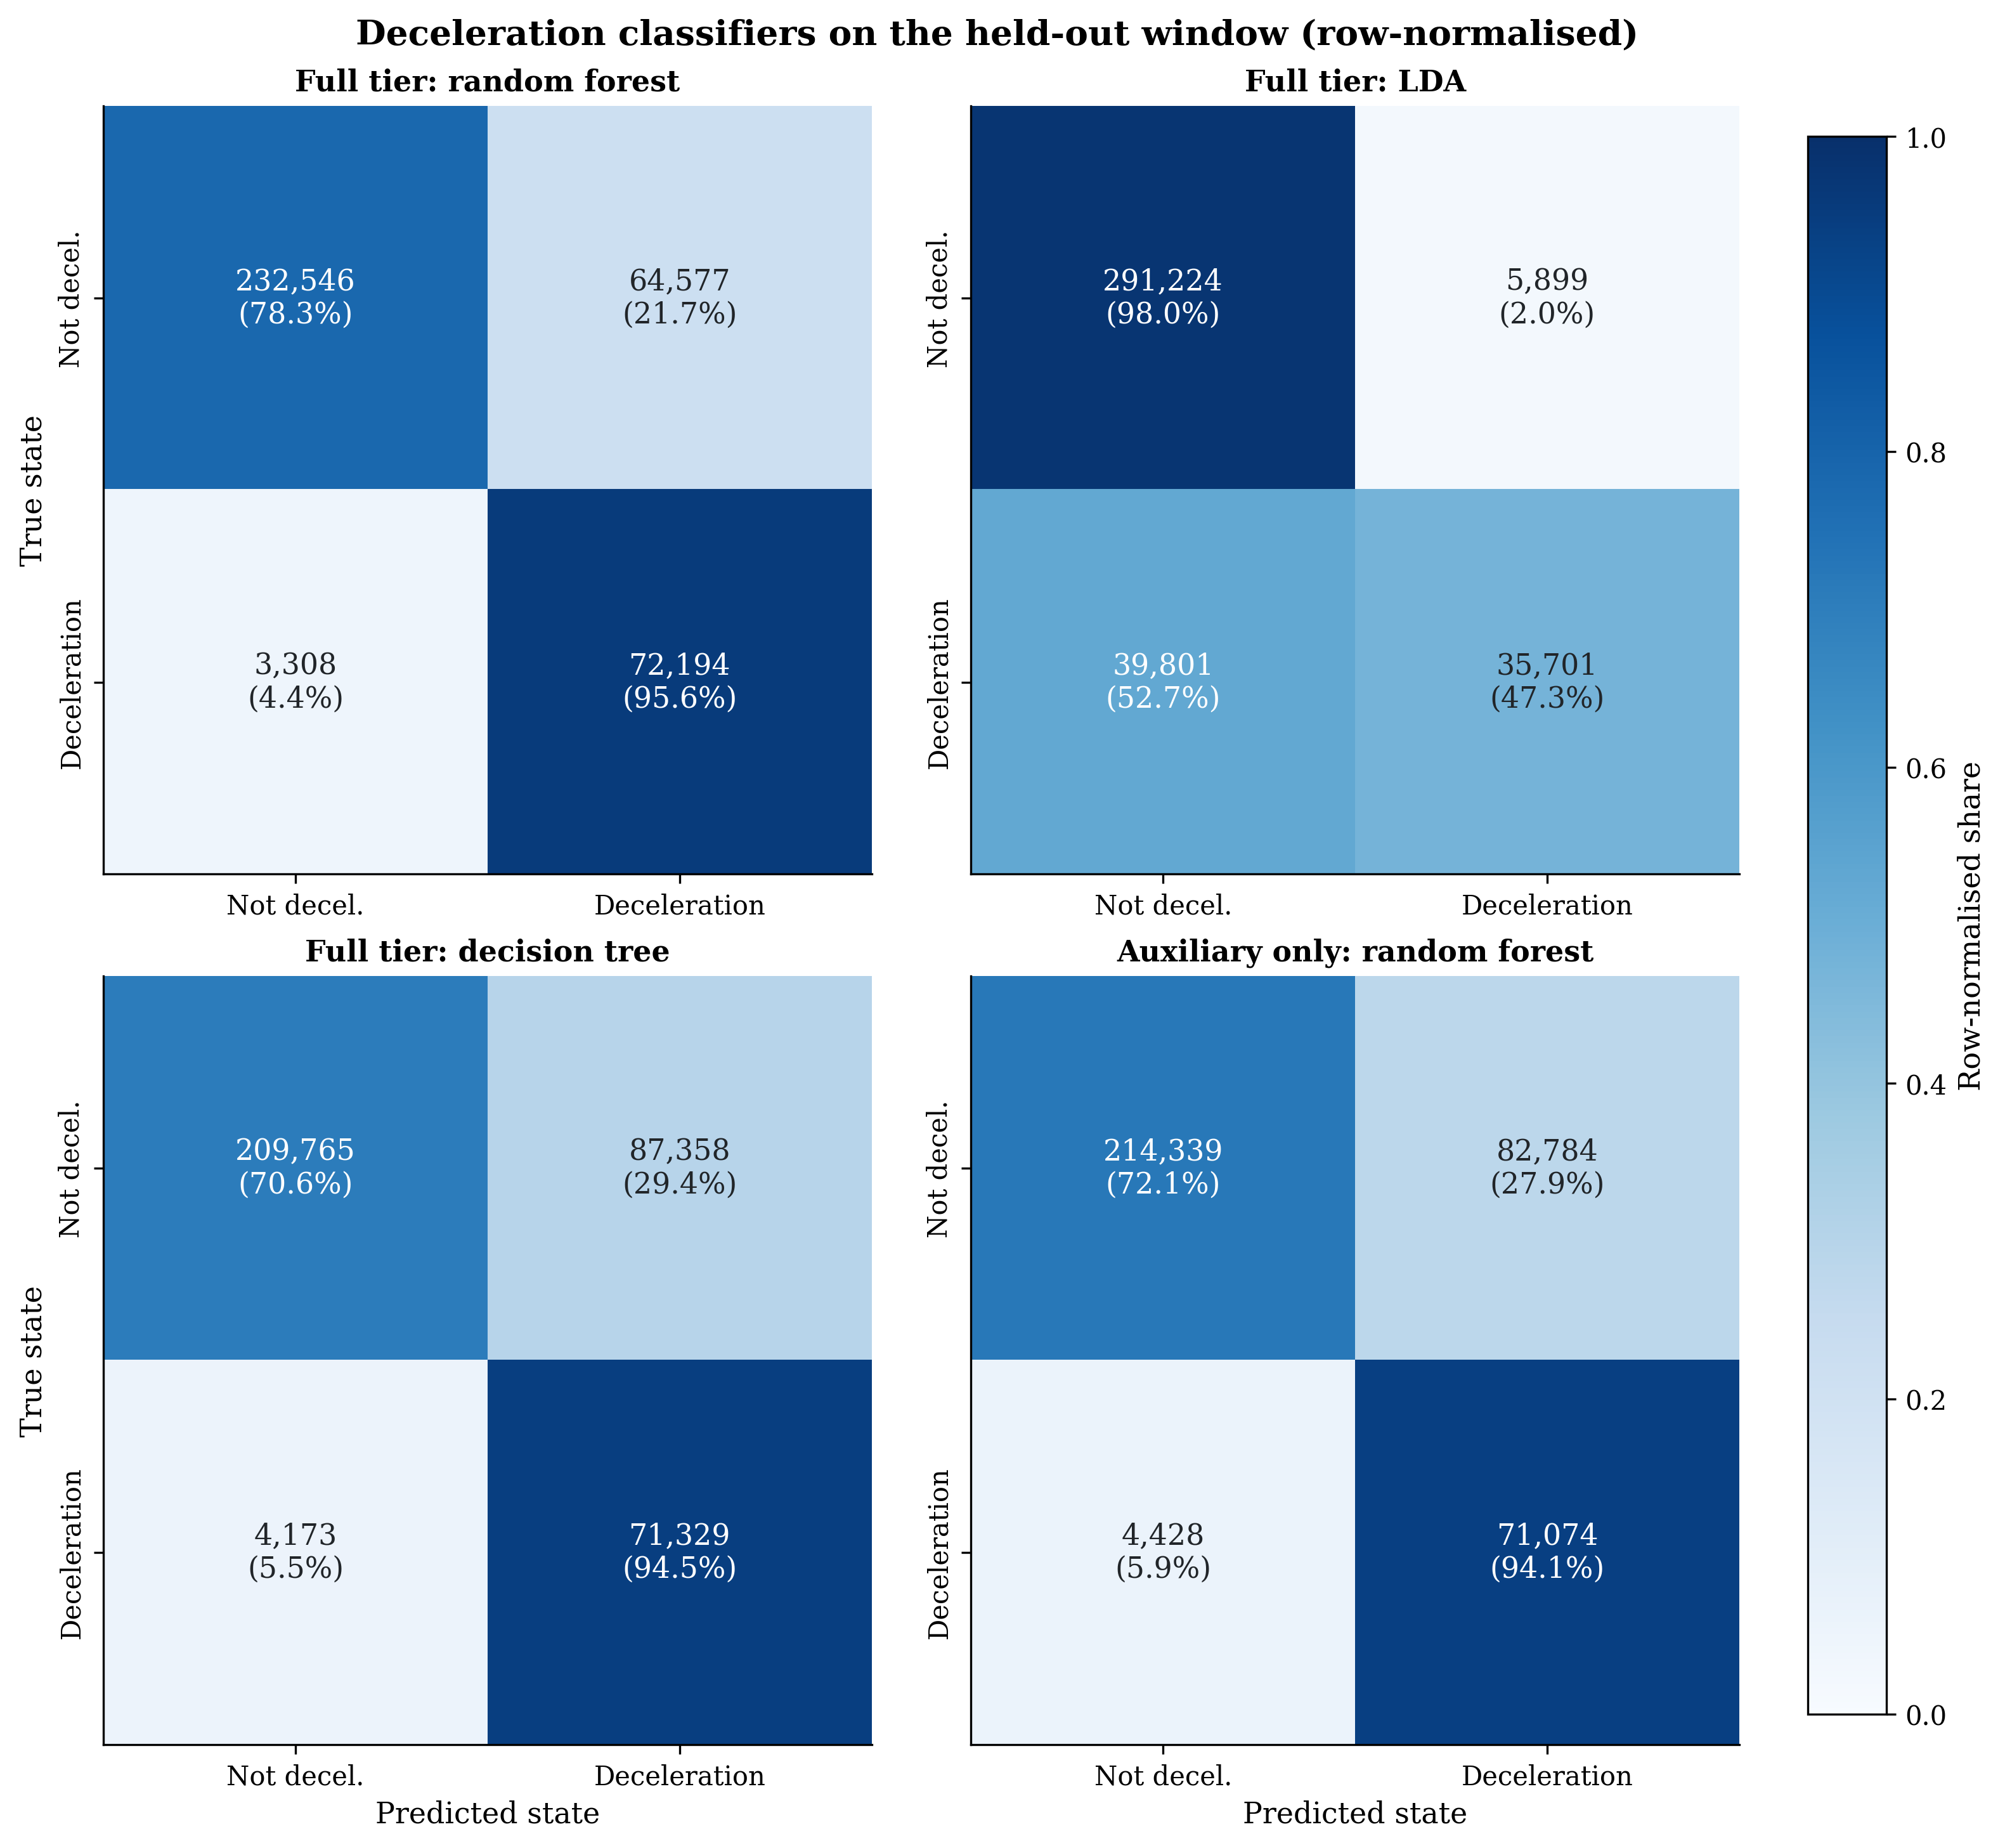
\includegraphics[width=0.85\linewidth]{state_clf_confusion.png}
  \caption{The four most informative confusion matrices on the held-out window
  (row-normalised). The full-tier random forest catches almost every deceleration at the
  cost of some false positives; LDA is the opposite, precise but conservative; the decision
  tree sits between them; and the auxiliary-only random forest, with the brake command
  withheld, keeps the same shape, showing the signal survives without actuation channels.}
  \label{fig:confusion}
\end{figure}

\chapter{Analysis of braking events}
\label{ch:braking}


\section{Events}

A deceleration event is one continuous stretch of the deceleration state; the training window
yields about 126{,}700, of which 99.9\% are genuine decelerations once the held-brake
contamination was removed (Section~\ref{sec:heldbrake}). The mean event lasts 23.4\,s and the
median 20\,s (95th percentile 30\,s): mostly ordinary station stops, with a thin tail of longer
ones.

\section{Classes or continuum?}
\label{sec:continuum}

The original plan anticipated discrete braking classes: light, hard, emergency. The data was
allowed to decide instead. Clustering the intensity features and reading BIC, silhouette, and
resampling stability together turns up no natural class count: the BIC keeps improving as
clusters are added rather than settling at a minimum, and the silhouette never singles out a $k$
(Figure~\ref{fig:continuum}). Stability does rise again at $k=5$, which looks stable at a glance
but survives only by peeling off a cluster holding a few hundredths of a percent of the events,
unsupported by BIC or silhouette: the bump is an artefact of one tiny outlier group, not a regime.
The intensity histogram seems to pull the other way, with a dominant mild mode and a broader hump
at firmer braking (Figure~\ref{fig:intensity}), so on its own the density looks bimodal. But the
humps overlap without a clean gap, and the resampling scrambles any boundary drawn between them,
so the clustering never confirms the visual split. That tension is left as an open question; on
the available evidence the report treats intensity as a continuum, varying by degree rather than
by kind. No light/hard/emergency labels are introduced, then. Any such split is an \emph{operational
threshold} to be set with domain input, not a structure the data volunteers.

\begin{figure}[htbp]
  \centering
  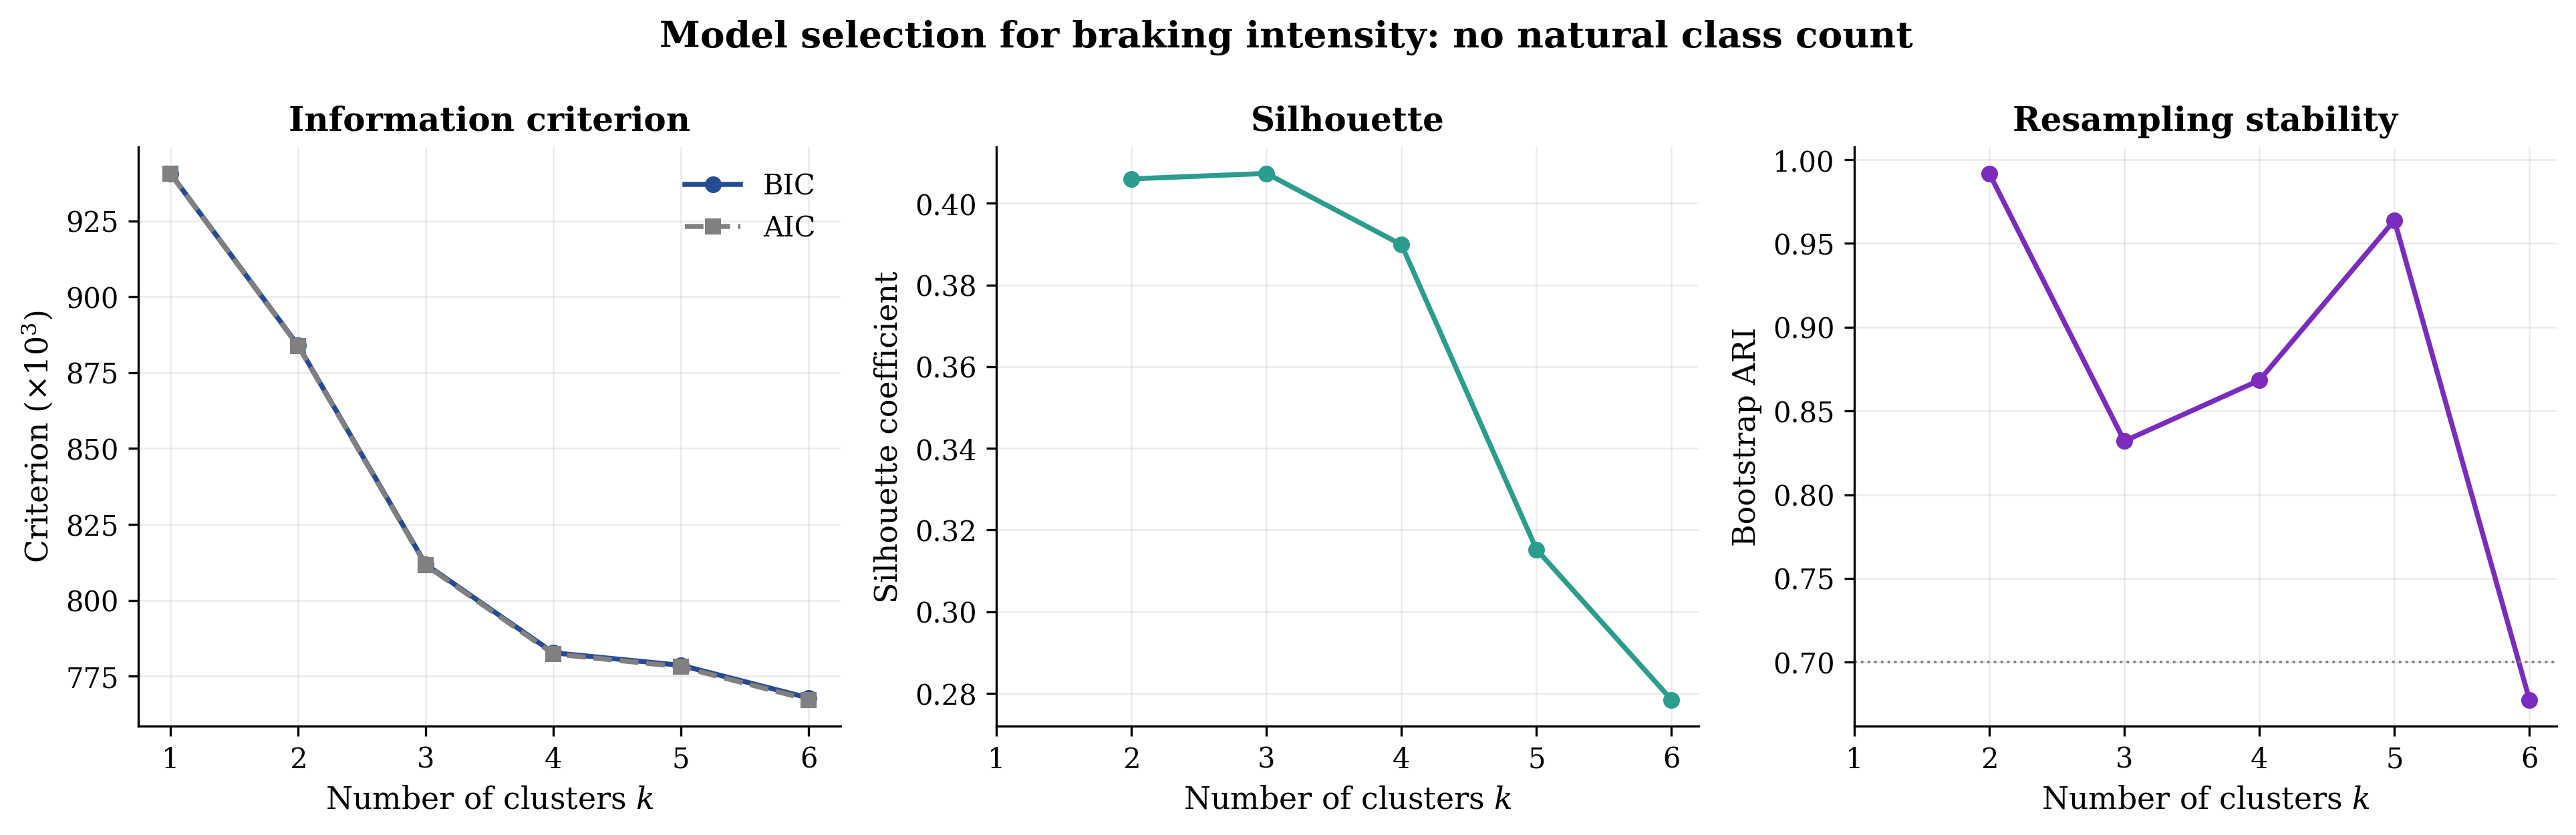
\includegraphics[width=\linewidth]{cluster_model_selection.png}
  \caption{Model selection for braking intensity. BIC keeps improving with more groups and
  the silhouette falls away, so there is no natural number of intensity classes. The
  resampling stability rises again at $k=5$, but that solution only splits off a negligibly
  small cluster and no other criterion supports it, so the bump carries no interpretable
  meaning: intensity is a continuum.}
  \label{fig:continuum}
\end{figure}

\begin{figure}[htbp]
  \centering
  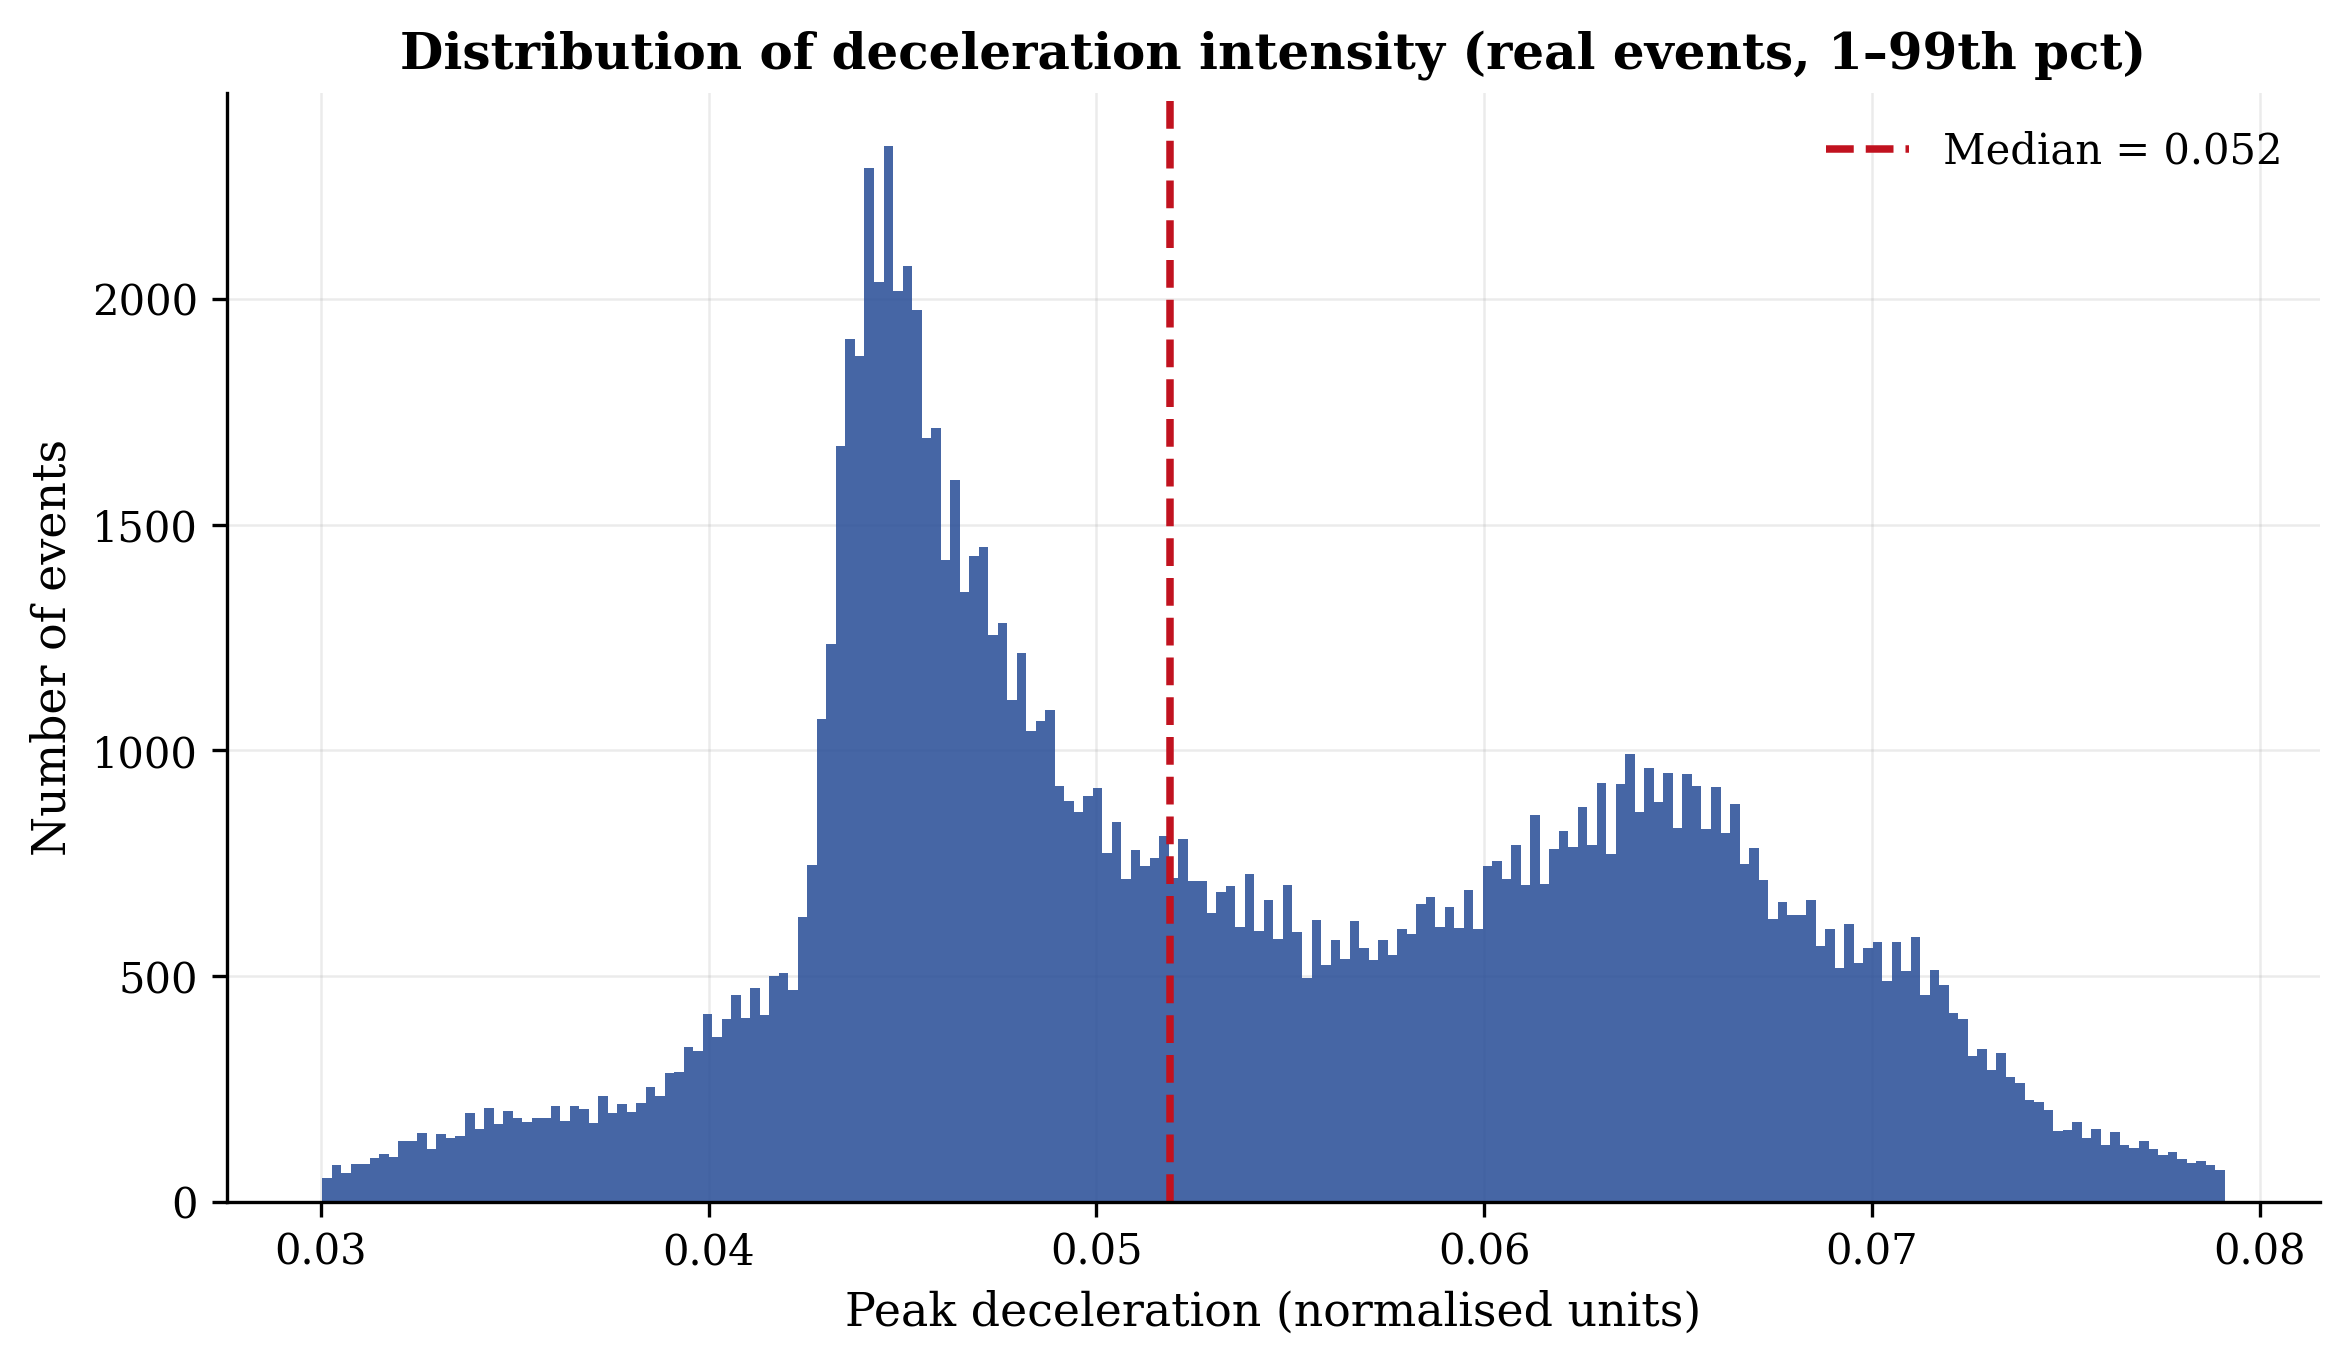
\includegraphics[width=1\linewidth]{intensity_distribution.png}
  \caption{Distribution of deceleration intensity. A dominant mild mode and a broader
  firmer-braking hump overlap without a clean gap; the cluster tests find no stable boundary
  between them, so intensity is treated as a continuum rather than as discrete classes.}
  \label{fig:intensity}
\end{figure}

\section{A deceleration-energy axis}
\label{sec:energy}

To compare stops on a physical scale, a specific deceleration energy is derived,
$\tfrac{1}{2}(v_0^2 - v_1^2)$, the kinetic energy dissipated per stop per unit mass. Being
kinematic, it carries the role \emph{velocity} and serves only as a target, never a predictor.
Adding it to the intensity features does not create classes (the continuum of
Section~\ref{sec:continuum} is unchanged) but gives a common wear axis, putting every stop on the
same energy-dissipated scale. The air-system sensors explain about 85\% of a stop's specific
energy out-of-sample (full tier, random forest), so the pneumatic record tracks dissipated energy
closely even without seeing the speed.

\section{Intensity regression}
\label{sec:regression}

The central cross-modal test predicts deceleration \emph{magnitude} from the non-speed sensors on
held-out events, against a guess-the-average baseline ($R^2 \approx 0$ by construction). A random forest on the full tier reaches $R^2 \approx 0.43$ for peak and $0.57$ for mean
deceleration; a linear model manages only 0.24 and 0.20, so most of the signal is non-linear
structure a straight fit misses. These are moderate results: the pneumatic sensors carry real but
partial information about how hard the train braked, not a near-perfect reconstruction. The scatter of predicted against actual intensity (Figure~\ref{fig:regscatter}) is positively
associated but sits in a narrower band than the targets: the gentlest stops are pushed up and the
hardest pulled down, flattening the cloud against the diagonal. This is regression toward the
average, where a squared-error model retreats when the inputs leave real variance unexplained, and
the per-event pneumatic signal is that noisy. Two other explanations were checked and rejected. Not sensor saturation: the actuation pressures
stay well inside range on hard stops, with only one to two percent of events near a ceiling. Not
the ten-second windowing either: adding event duration to the predictors moves $R^2$ by less than
a percentage point. The model did matter. A gradient-boosted tree scores 0.47 on mean deceleration
in a tighter band; the random forest reaches 0.57 and widens the spread by about a fifth, since
deep independent trees reach more extreme conditional means than a shallow boosted ensemble. Peak
deceleration holds at 0.43 either way, so its residual band is the limit of what these sensors
carry, not a model shortcoming. Both panels of Figure~\ref{fig:regscatter} use the random forest. A Lasso fit with its penalty cross-validated on the training events keeps 19 of the 22 air-system
features ($\alpha \approx 4\times10^{-6}$), a mix of actuation and auxiliary channels spread across
subsystems rather than concentrated in the brake command. The near-minimal penalty and broad
selection say the intensity signal is distributed, not localised, matching the auxiliary-only
classification result of Chapter~\ref{ch:classification}.

\begin{figure}[htbp]
  \centering
  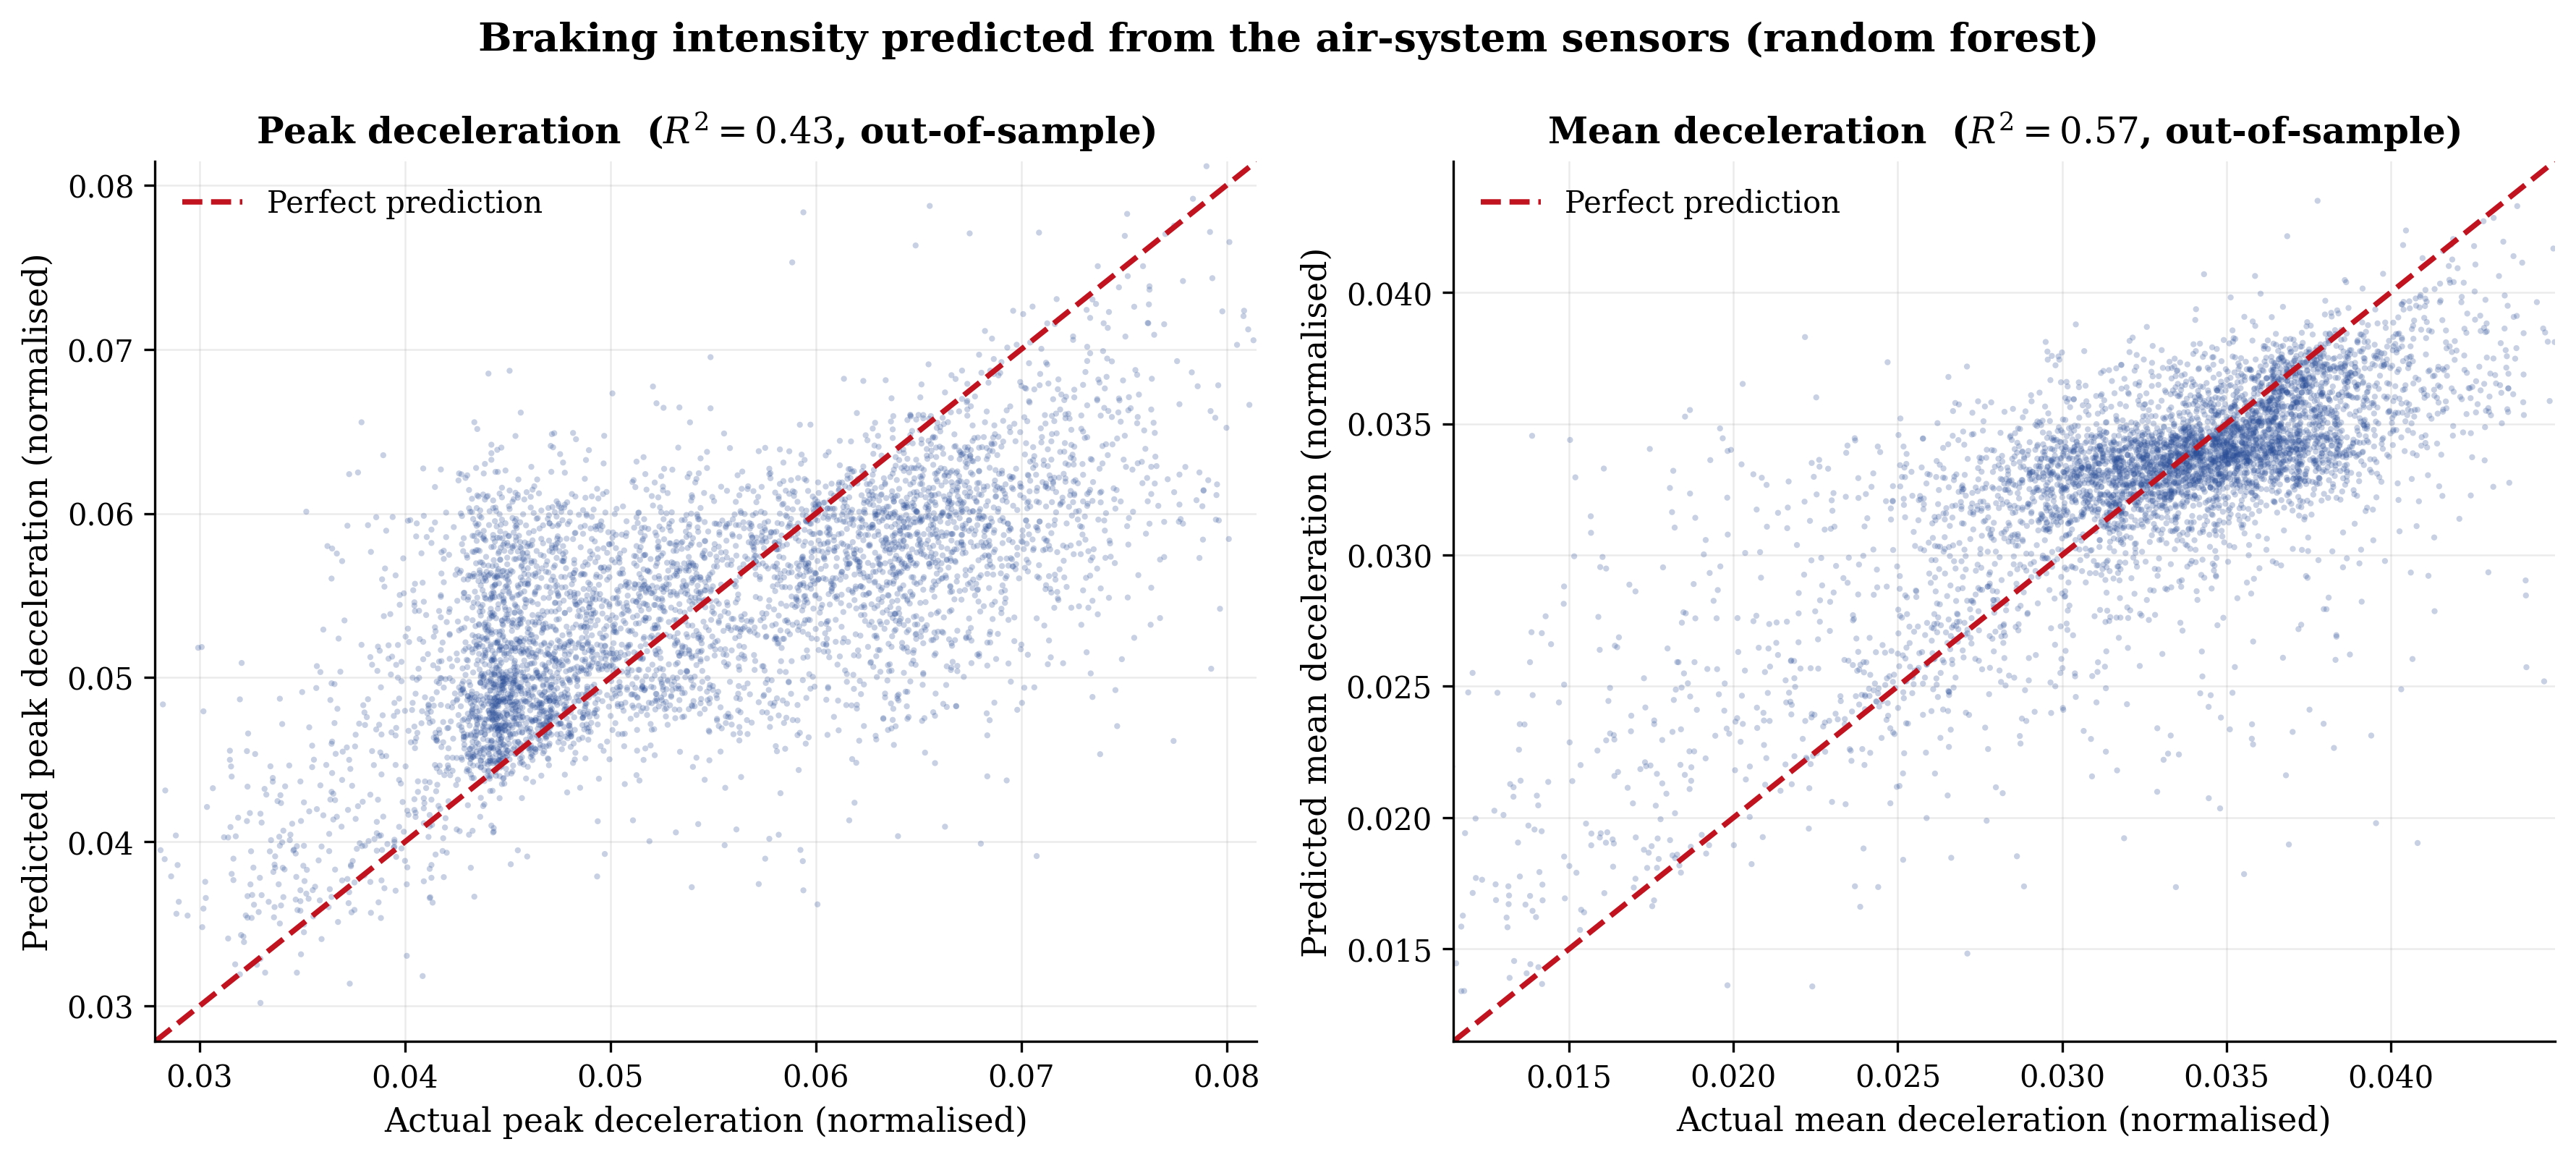
\includegraphics[width=\linewidth]{decel_regression_scatter.png}
  \caption{Predicted versus actual deceleration intensity on held-out events (full tier,
  random forest). The association is positive, but predictions sit in a narrower band than
  the targets: the gentlest stops are over-predicted and the hardest under-predicted, the
  regression-toward-the-average that remains once the pneumatic sensors have given up their
  partial signal.}
  \label{fig:regscatter}
\end{figure}

\chapter{Connection to failure events and maintenance}
\label{ch:failure}

The preceding chapters established that motion defines four operational states, that the
air-system sensors independently recover the deceleration state, and that they explain a
moderate share of braking intensity. This chapter turns to the question behind predictive
maintenance: does braking behaviour change in the days before a documented brake-system failure?
The evidence points to a near-null answer, reported here as a genuine negative rather than
qualified away.

\section{Setup}

The training window contains 10 documented failures (8 brake-system) and 11 maintenance events.
Deceleration events in the seven days before any brake failure form a pre-failure group (about
23{,}000 events), compared against a baseline more than 30 days from any failure (about 44{,}000).
Ten event-level features are tested, spanning the kinematic intensity measures and the auxiliary
health channels.

\section{Distributional test}
\label{sec:prefailure-test}

Each feature is compared between the pre-failure and baseline groups with a Mann--Whitney $U$
test~\cite{MannWhitney:47}, a rank-based test that asks whether values from one group tend to exceed the other without
assuming normality: it ranks the pooled values and counts, over every cross-group pair, how often
the pre-failure value is larger. Under the null that count is about $n_1 n_2 / 2$, and the
$p$-value measures the departure from it. With ten features tested, the $p$-values are
Bonferroni-corrected: at $m=10$ and $\alpha = 0.05$ a feature counts as significant only if its
raw $p$ falls below $\alpha/m = 0.005$, capping the family-wide false-positive chance at $\alpha$.
With more than 23{,}000 pooled events almost every feature clears that bar, which means little
here: at this sample size even trivial differences drive $p$ to zero. What is read instead is the
effect size, Cliff's delta~\cite{Cliff:93}, where $0$ is no separation and $\pm 1$ total, with $|\delta| < 0.15$
treated as negligible.

The result is near-null (Table~\ref{tab:prefailure}). The kinematic and braking-command features
(peak and mean deceleration, deceleration energy, brake-cylinder and pneumatic-braking-force
channels) all sit at $|\delta| < 0.06$, effectively no separation despite significant $p$-values.
Only energy-braking-resistance clears the threshold, at $|\delta| \approx 0.20$; the next largest,
load pressure at $\approx 0.10$, stays negligible. Even that effect is small and rests on only
eight brake failures, so it cannot support a prediction claim on its own. It does hint at
\emph{where} any signal might live, in the auxiliary channels rather than the deceleration
kinematics, a point the conclusion returns to.

\begin{table}[htbp]
  \centering
  \caption{Pre-failure versus baseline effect sizes (Cliff's delta), top 7 $|\delta|$
  values. The braking-kinematic features are negligible; only one auxiliary channel
  (energy-braking-resistance) rises above $|\delta| = 0.15$, and even that is small and rests
  on eight brake failures. Negative $\delta$ means lower values before failure.}
  \label{tab:prefailure}
  \begin{tabular}{lrc}
    \toprule
    Feature & Cliff's $\delta$ & Above negligible ($|\delta|>0.15$)? \\
    \midrule
    energy-braking-resistance (mean)   & $-0.201$ & yes \\
    load pressure (mean)               & $-0.103$ & no  \\
    jerk RMS                           & $+0.054$ & no  \\
    brake-cylinder pressure (integral) & $-0.040$ & no  \\
    deceleration energy (specific)     & $-0.039$ & no  \\
    pneumatic braking force (mean)     & $-0.032$ & no  \\
    peak deceleration                  & $-0.005$ & no  \\
    \bottomrule
  \end{tabular}
\end{table}

\section{Change-point detection}
\label{sec:changepoint}

As an independent check, a CUSUM (cumulative-sum) change-point detector~\cite{Page:54} was run on the strongest
signal from the previous section, the weekly mean of energy-braking-resistance
(Figure~\ref{fig:cusum}). One design choice matters here and applies to this figure alone. The raw
weekly proxy climbs almost monotonically across the year, which would only make sense if brake wear
never reversed. Assuming the brakes are serviced, the proxy is reset to its post-service level at
every maintenance date and only the within-interval drift is read. This is an assumption, not a
fact: the log records that a stop happened, not that the brakes were touched, so the reset may not
hold at every stop. It is adopted because a proxy that only ever rises is not sensible to run a
change-point test on.

CUSUM keeps a running total of each week's deviation from the established mean: while the process
is stable the positive and negative deviations cancel and the sum stays near zero, but once the
level shifts they share a sign and the sum climbs until it crosses a threshold and flags a
change-point. A persistent drift thus surfaces where one-off noise does not. The threshold is four
standard deviations, tuned for about one false alarm every six months. On the reset signal it
fires four times, only one within seven days of a documented failure. There is no reliable
alignment between change-points and failures during the deceleration phase, consistent with the
near-null effect sizes of Section~\ref{sec:prefailure-test}.

\begin{figure}[htbp]
  \centering
  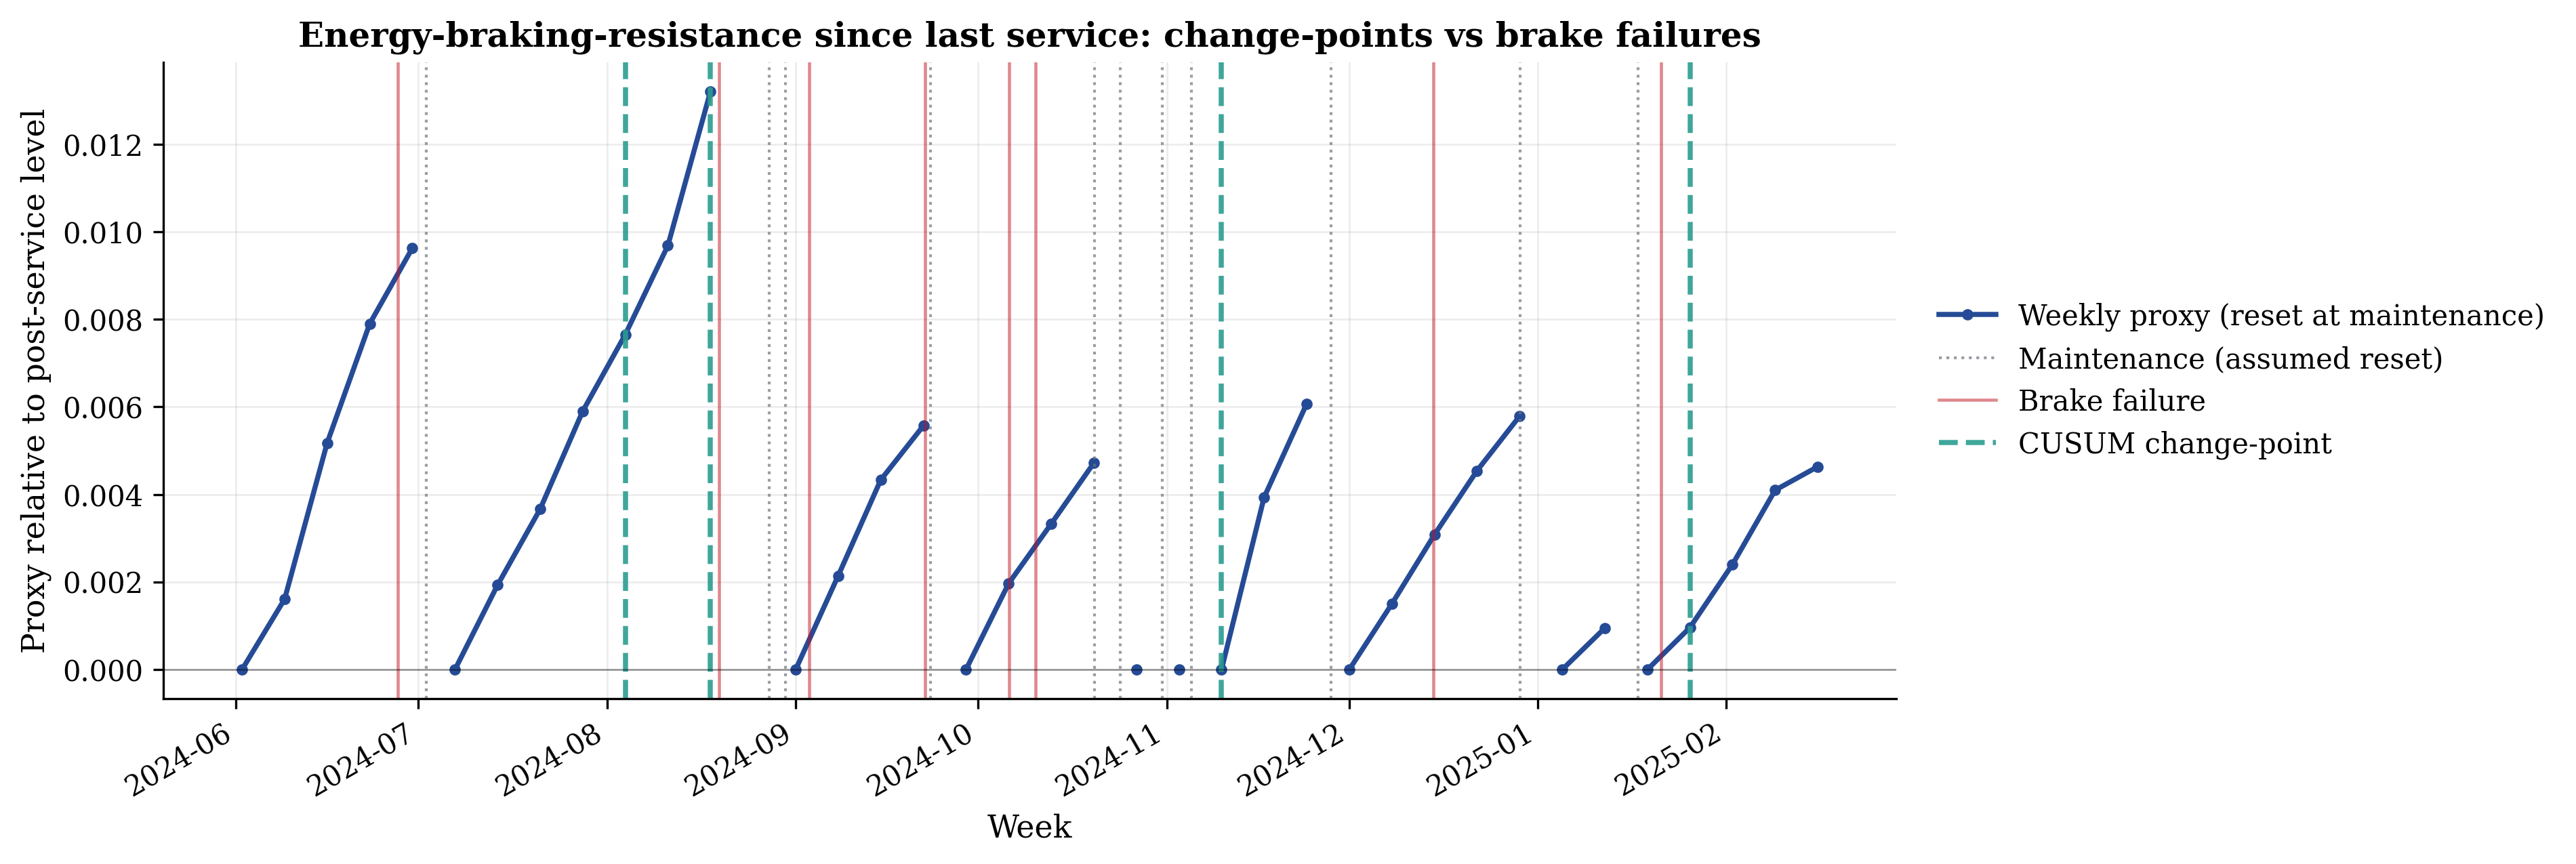
\includegraphics[width=0.95\linewidth]{prefailure_cusum.png}
  \caption{CUSUM change-points on the weekly mean of energy-braking-resistance, the auxiliary
  channel with the largest pre-failure effect size, reset to its post-service level at each
  maintenance date (dotted) under the assumption that the brakes are serviced there. Within
  each between-maintenance interval the proxy drifts up from zero; four change-points fire and
  only one falls within seven days of a documented failure, so even the strongest proxy does
  not track failures during the deceleration phase.}
  \label{fig:cusum}
\end{figure}

\section{Energy and the maintenance calendar}

The deceleration-energy axis of Section~\ref{sec:energy} was examined descriptively against the
maintenance calendar (Figure~\ref{fig:maint}). Energy totals track how long an interval ran and how
much the train moved, following interval length more than failure risk. A CUSUM on weekly summed
energy fires three times, again only one within seven days of a failure. As an accounting check,
about 96\% of all real-deceleration energy falls inside the between-maintenance intervals, so
almost no braking is missed.

One pattern in the same figure is worth flagging, with care. Every between-maintenance interval
containing a brake failure ran longer than about three weeks, and every shorter one was
failure-free: the groups separate cleanly at roughly 21 days. On the service-at-each-stop reading
of Section~\ref{sec:changepoint}, a longer unmaintained stretch gives wear more time to build,
which would make a cadence under three weeks a sensible target. Two cautions hold. A longer
interval also spans more calendar days, so it has more chance to contain any event at all,
confounding length with exposure; and the pattern rests on ten intervals and eight brake failures.
It is an idea worth testing on more data, not a result.

\begin{figure}[htbp]
  \centering
  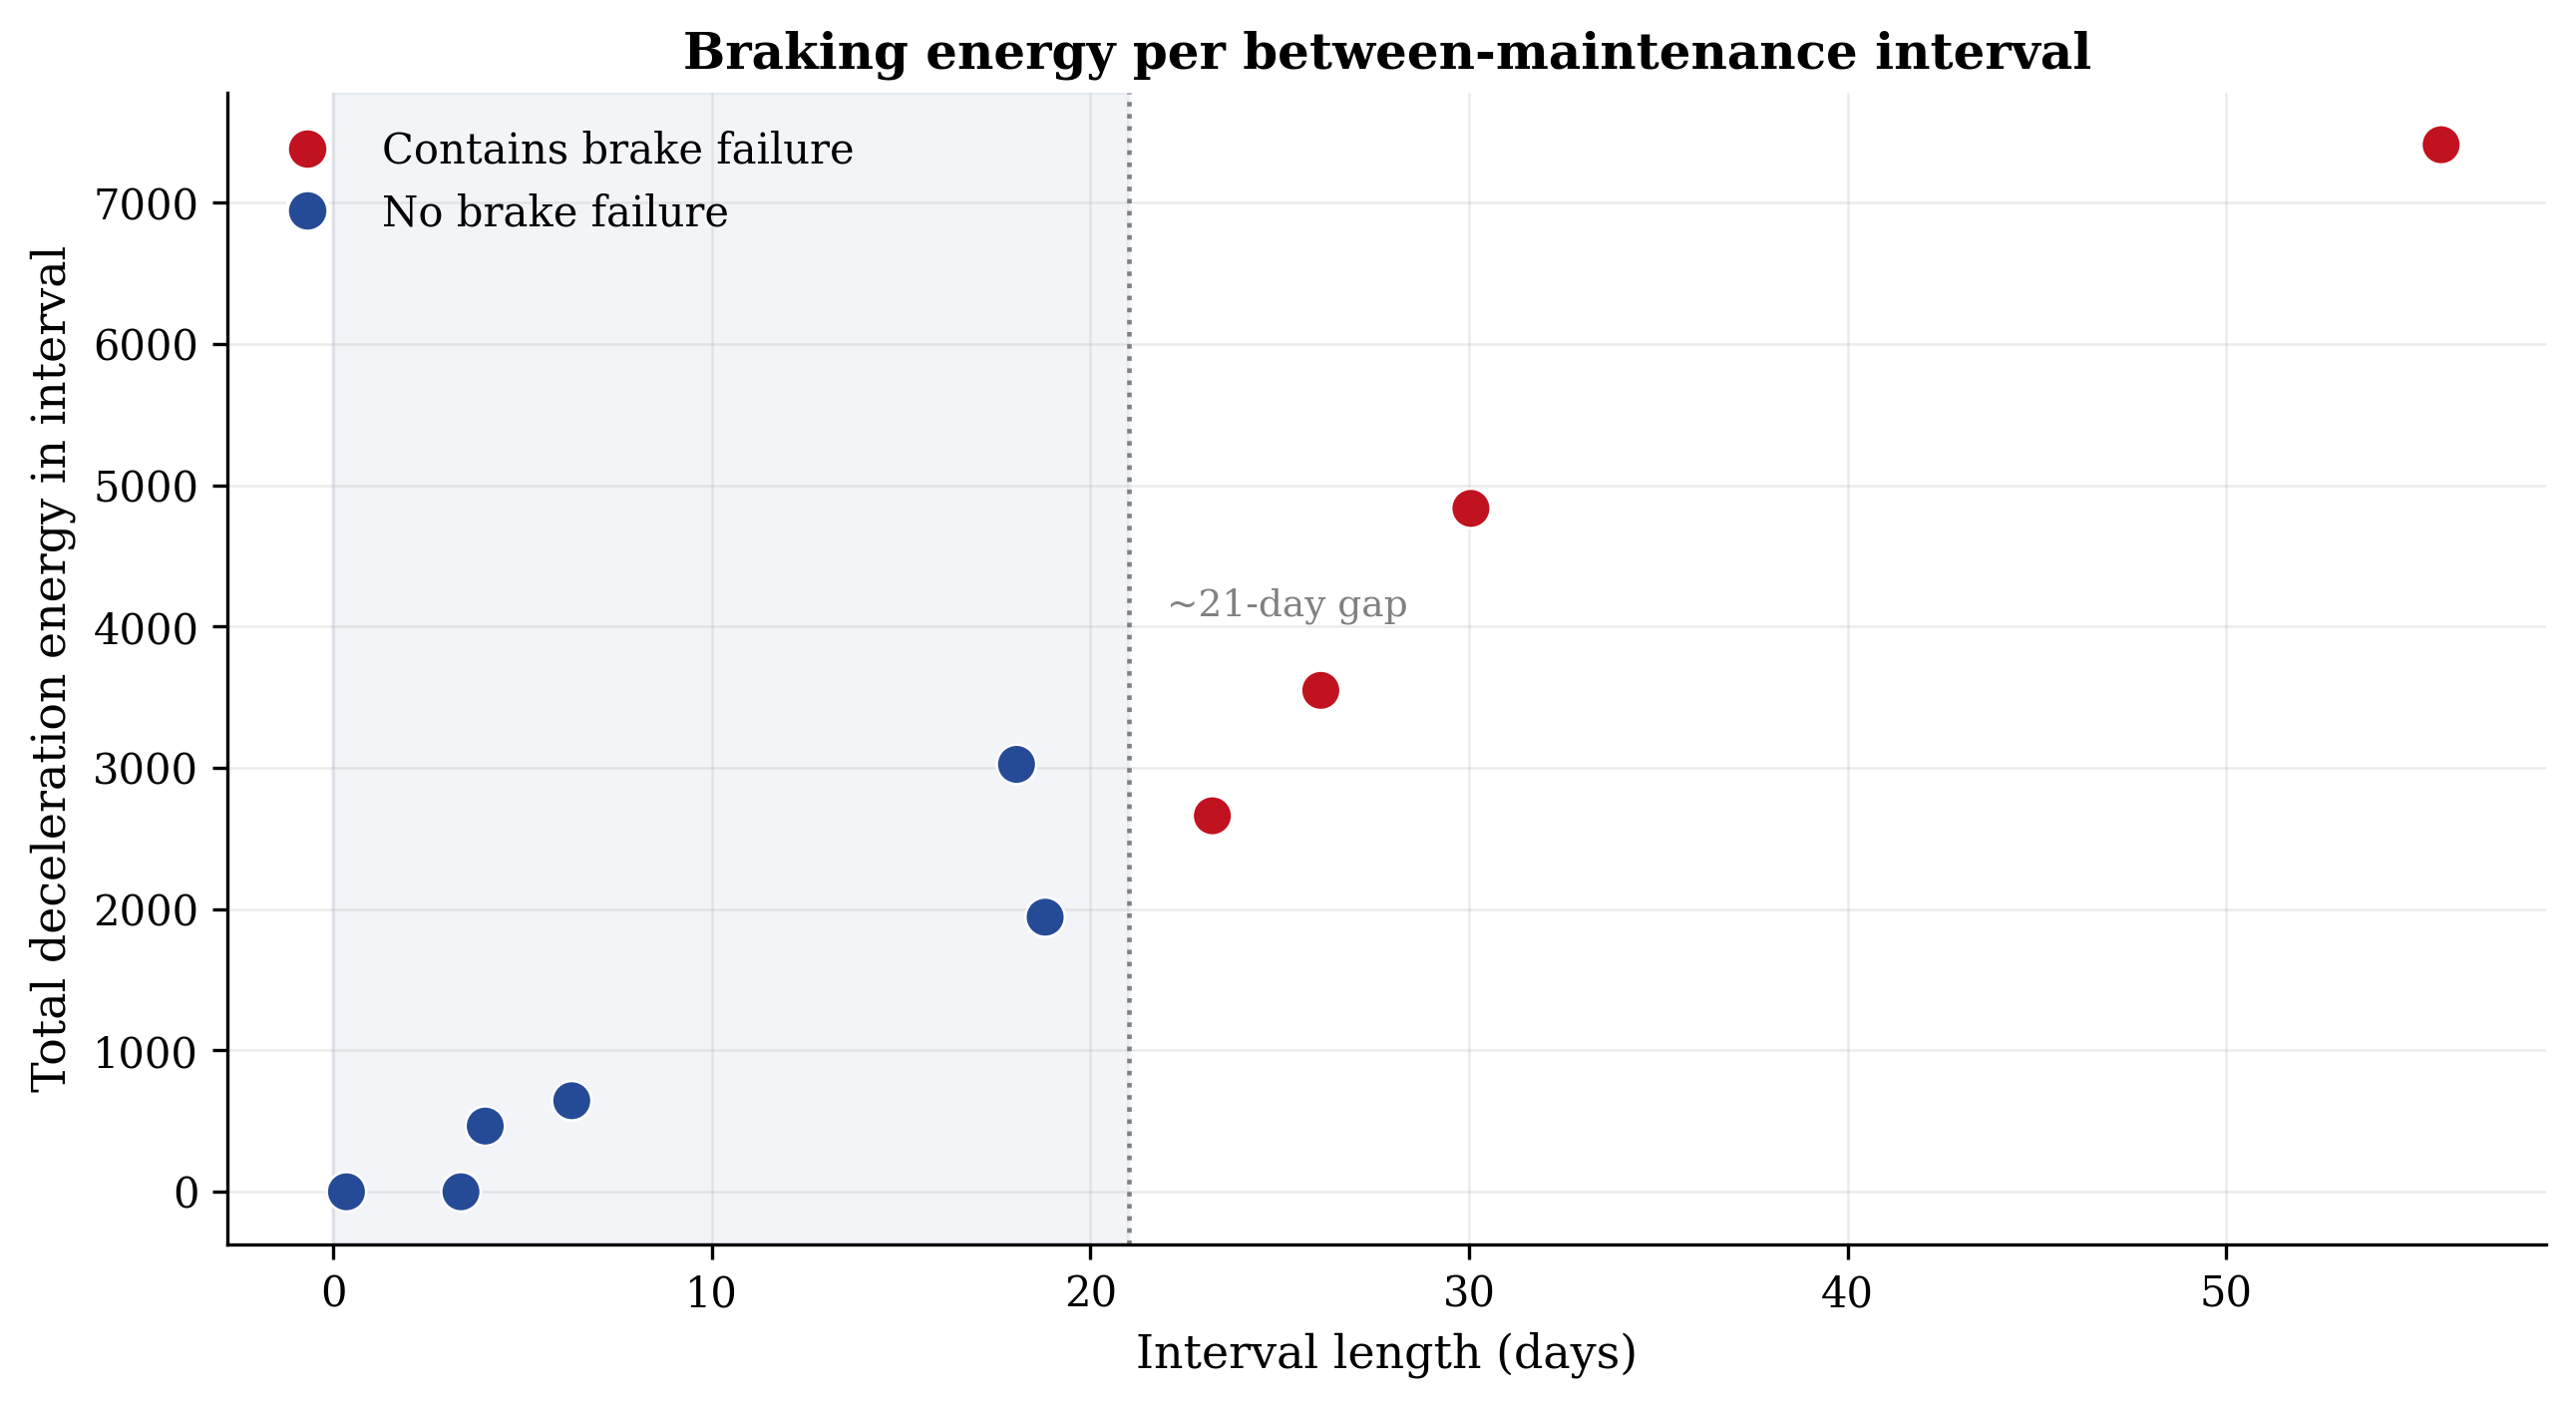
\includegraphics[width=0.9\linewidth]{maintenance_interval_energy.png}
  \caption{Deceleration energy per between-maintenance interval. Totals rise with interval
  length. Every interval that contained a brake failure (red) ran longer than about three
  weeks; every shorter interval was failure-free. The split is suggestive but confounded with
  exposure time and rests on ten intervals.}
  \label{fig:maint}
\end{figure}

\chapter{Conclusion}
\label{ch:conclusion}

Motion alone splits a year of running into four operational states (standing, accelerating,
cruising, deceleration), and the air-system sensors, held out of that definition, recover the
deceleration state on their own: a random forest reaches ROC-AUC 0.95 on held-out data, and
0.92 even with the brake command withheld. Deceleration therefore leaves an independent
fingerprint across the pneumatic system. Its intensity is a continuum rather than a set of
classes, and the same sensors explain a moderate share of it out-of-sample (peak $R^2 \approx
0.43$, mean $0.57$) and about 85\% of a stop's dissipated energy. The link to failures is an
honest negative: neither the effect-size tests, the change-point detector on the strongest
channel, nor the energy-versus-maintenance view separates the pre-failure period from baseline
at only eight brake failures. Two soft hints survive, a small residual effect in the auxiliary
channels rather than the braking kinematics, and a clean split in which every maintenance gap
longer than about three weeks coincided with a failure. Both point to where a future search
might look; neither is a detector.

The one open method question from Chapter~\ref{ch:braking} is now settled. Cross-validating
the Lasso penalty (five-fold, on the training events only, so no held-out data leaks into the
choice) selects a small penalty ($\alpha \approx 4\times10^{-6}$) and keeps 19 of the 22
air-system channels. The intensity signal is spread across subsystems, not carried by the
brake command alone.

Four directions follow, three concrete and one broad. First, the off-curve outliers in the
velocity--acceleration cycle (Section~\ref{sec:fourstates}) were never characterised and may
flag unusual operating conditions. Second, the per-wagon sensor copies were collapsed rather
than compared; differences between wagons could localise where wear develops. Third, the
pre-failure tests should be repeated on the standing and cruising states, where charging and
idle behaviour (compressor duty cycle, reservoir recharge, spring-brake pressure at rest) is
most visible and where brake faults are likeliest to actually show. Underlying all three is
the reason none of them is guaranteed to pay off: this study found no dependable indicator of
physical wear, and a dataset with many more documented failures is what would let any of these
turn a hint into evidence.

The full pipeline, from raw recordings to the figures and tables in this report, is available
on GitHub so the analysis can be reproduced end to end.\footnote{\url{https://github.com/maxscheiblauer/Interdisciplinary_Project}}

\printbibliography[heading=bibintoc]
% =========================================================================
%  Appendix
% =========================================================================
\appendix
\chapter{Feature roles}
\label{app:roles}

This appendix lists the assignment of MetroAT channels to the feature roles introduced in
Section~\ref{sec:roles}. Only \emph{actuation} and \emph{auxiliary} channels are eligible as
predictors; \emph{velocity} channels define the targets, and \emph{other} channels are used
only for the train/held-out split, time alignment, and validation. Pneumatic channels are
replicated per wagon (for example \texttt{\ldots\_BOGIE1}, \texttt{\ldots\_BOGIE2}); each entry
below stands for the whole family of per-wagon copies, which are collapsed by principal
component analysis (Figure~\ref{fig:pca}) where a compact input is required. The exhaustive,
machine-readable assignment is stored in \texttt{feature\_roles.csv}.

\begin{table}[htbp]
  \centering
  \caption{Assignment of MetroAT channels to feature roles.}
  \label{tab:approles}
  \begin{tabularx}{\linewidth}{l l >{\RaggedRight}X}
    \toprule
    Role & Predictor & Channels \\
    \midrule
    velocity  & no  & train speed (\texttt{TRAIN\_SPEED\_ACTUAL}) and the derived acceleration,
                      jerk, velocity-change-rate, and deceleration-energy features \\[1ex]
    actuation & yes & brake-cylinder pressure, proportional-valve pressure
                      (\texttt{*\_PROPORTIONAL\_VALVE\_PRESSURE\_*}), spring-brake pressure, and
                      pneumatic braking force (\texttt{*\_PNEUMATIC\_BRAKING\_FORCE\_*}) \\[1ex]
    auxiliary & yes & main-reservoir pressure, load pressure, load signal,
                      energy-braking-resistance, ambient temperature, and compressor-running \\[1ex]
    other     & no  & timestamps, operating-mode flags (\texttt{TRAIN\_*\_MODE}), and the
                      failure and maintenance markers (\texttt{TRAIN\_IS\_IN\_FAILURE},
                      \texttt{TRAIN\_IS\_IN\_MAINTENANCE}, \texttt{TRAIN\_FAILURE\_TYPE},
                      \texttt{TRAIN\_MAINTENANCE\_TYPE}) \\
    \bottomrule
  \end{tabularx}
\end{table}

\section{Kinematic features}
\label{app:kinematics}

The operational states of Chapter~\ref{ch:states} are clustered from kinematic
(\emph{velocity}-role) features alone. These rest on a single raw channel from the dataset,
the train speed, from which acceleration, its absolute rate, and jerk are derived on the
time-sorted 1\,Hz stream. All derivatives are $\Delta t$-aware (they use the actual time gap
between consecutive samples) and are set to zero across gaps longer than 2\,s, so that
out-of-service breaks do not create spurious spikes. Table~\ref{tab:kinematics} lists the four
base signals with their origin and, where derived, their formula. Here $v_t$ is the normalised
speed at sample $t$ and $\Delta t$ the interval to the previous sample (nominally 1\,s).

\begin{table}[htbp]
  \centering
  \caption{The kinematic base signals: origin (raw dataset channel versus crafted) and, for the
  crafted signals, their definition. All values are in the normalised units of the dataset;
  rates are per second.}
  \label{tab:kinematics}
  \begin{tabularx}{\linewidth}{l l >{\RaggedRight}X}
    \toprule
    Signal & Origin & Definition \\
    \midrule
    train speed $v$ & dataset & raw channel \texttt{TRAIN\_SPEED\_ACTUAL}, min-max normalised
      to $[0,1]$ \\[0.6ex]
    acceleration $a$ & crafted & $a_t = \dfrac{v_t - v_{t-1}}{\Delta t}$ \\[1.2ex]
    velocity-change rate & crafted & $\left| a_t \right| = \left| \dfrac{v_t - v_{t-1}}{\Delta t}
      \right|$, the unsigned acceleration \\[1.2ex]
    jerk $j$ & crafted & three-sample rolling mean of $\dfrac{a_t - a_{t-1}}{\Delta t}$
      (the smoothed rate of change of acceleration) \\
    \bottomrule
  \end{tabularx}
\end{table}

Each base signal is reduced to per-window summaries over the ten-second window. The clustering
uses twelve window features: the mean and standard deviation of all four signals (eight
features), together with the minimum and maximum of speed and of acceleration (four features).
The event-level kinematic descriptors used for braking intensity in Chapter~\ref{ch:braking}
(peak and mean deceleration, $\Delta v$, jerk peak and RMS, and the two deceleration-energy
axes) are derived from the same speed channel and are defined where they are first used.
\chapter{Full classifier metrics}
\label{app:clfmetrics}

Table~\ref{tab:clfmetrics} reports every model scored in Chapter~\ref{ch:classification} on
the held-out window, for both predictor tiers. The main text quotes ROC-AUC, balanced
accuracy, and $F_1$; the precision and recall columns are added here to make the
precision/recall trade-off explicit. Deceleration is the minority class (about 20\% of
windows), so accuracy alone is misleading and balanced accuracy and ROC-AUC are the primary
yardsticks. All numbers are read directly from
\texttt{state\_classification\_metrics.csv}.

\begin{table}[htbp]
  \centering
  \caption{Deceleration classifiers on the held-out window, all models and both tiers,
  ordered by ROC-AUC within tier. Precision, recall, and $F_1$ are for the deceleration
  class.}
  \label{tab:clfmetrics}
  \begin{tabular}{llrrrrrr}
    \toprule
    Tier & Model & Acc. & Bal.\ acc. & Prec. & Recall & $F_1$ & ROC-AUC \\
    \midrule
    full & random forest      & 0.818 & 0.869 & 0.528 & 0.956 & 0.680 & 0.954 \\
    full & LDA                & 0.877 & 0.726 & 0.858 & 0.473 & 0.610 & 0.924 \\
    full & decision tree      & 0.754 & 0.825 & 0.449 & 0.945 & 0.609 & 0.910 \\
    full & logistic reg.      & 0.750 & 0.817 & 0.444 & 0.929 & 0.601 & 0.908 \\
    full & QDA                & 0.844 & 0.746 & 0.622 & 0.583 & 0.602 & 0.901 \\
    \midrule
    aux.\ only & random forest & 0.766 & 0.831 & 0.462 & 0.941 & 0.620 & 0.921 \\
    aux.\ only & decision tree & 0.731 & 0.796 & 0.424 & 0.906 & 0.577 & 0.878 \\
    aux.\ only & QDA           & 0.521 & 0.693 & 0.295 & 0.983 & 0.454 & 0.844 \\
    aux.\ only & logistic reg. & 0.719 & 0.728 & 0.397 & 0.744 & 0.517 & 0.814 \\
    aux.\ only & LDA           & 0.820 & 0.621 & 0.621 & 0.287 & 0.392 & 0.813 \\
    \bottomrule
  \end{tabular}
\end{table}


% =========================================================================
%  Bibliography
% =========================================================================


\end{document}
